%\documentclass[a4,semhelv,landscape]{seminar}
\documentclass[landscape]{slides}
%\documentclass[pdf, default, slideBW, nocolorBG]{prosper}
\usepackage[left=0.2cm,top=0.2cm,right=0.2cm,bottom=0.2cm,nohead,nofoot]{geometry}
%\def\everyslide{\sffamily}
%\usepackage{fullpage}
\usepackage{graphicx}
\usepackage[usenames]{color}
%\usepackage{color}
\usepackage{verbatim}
\usepackage{nopageno}
\usepackage{setspace}
%\usepackage{times}
% define some nice colors
\definecolor{myred}{rgb}{0.6,0,0}
\definecolor{myblue}{rgb}{0,0.2,0.4}
\definecolor{mygreen}{rgb}{0,0.5,0.0}
\definecolor{mypurple}{cmyk}{0.5,1.0,0.0,0.0}
%\color{myblue}

\begin{document}
%%%%%%%%%%%%%%%%%%%%%%%%%%%%%%%%%%%%%%%%%%%%%%%%%%%%%%%%%%%%%%%%%%%%
%Slide 0 - title
\begin{slide}
\begin{center}
\large{\textbf{Modeling Structural RNA Families \\ with Infernal}}

\normalsize

Eric Nawrocki

Sean Eddy's Lab

%10.05.11

\medskip

\medskip

\small

%\begin{tabular}{c}
%Howard Hughes Medical Institute \\ 
%Janelia Research Campus \\
%\\
%Deparment of Genetics \\
%Washington University in St. Louis \\
%\\
%\end{tabular}

%\vspace{0.1in}

%
\includegraphics[width=2.5in]{figs/janelia-logo}

\includegraphics[width=3in]{figs/jrc-color}
\end{center}
\end{slide}
%%%%%%%%%%%%%%%%%%%%%%%%%%%%%%%%%%%%%%%%%%%%%%%%%%%%%%%%%%%%%%%%%%%%
\begin{slide}
\begin{center}
{\bf Many functional RNAs adopt a conserved 3-dimensional 
  structure}

\medskip

Three representations of a transfer RNA:

%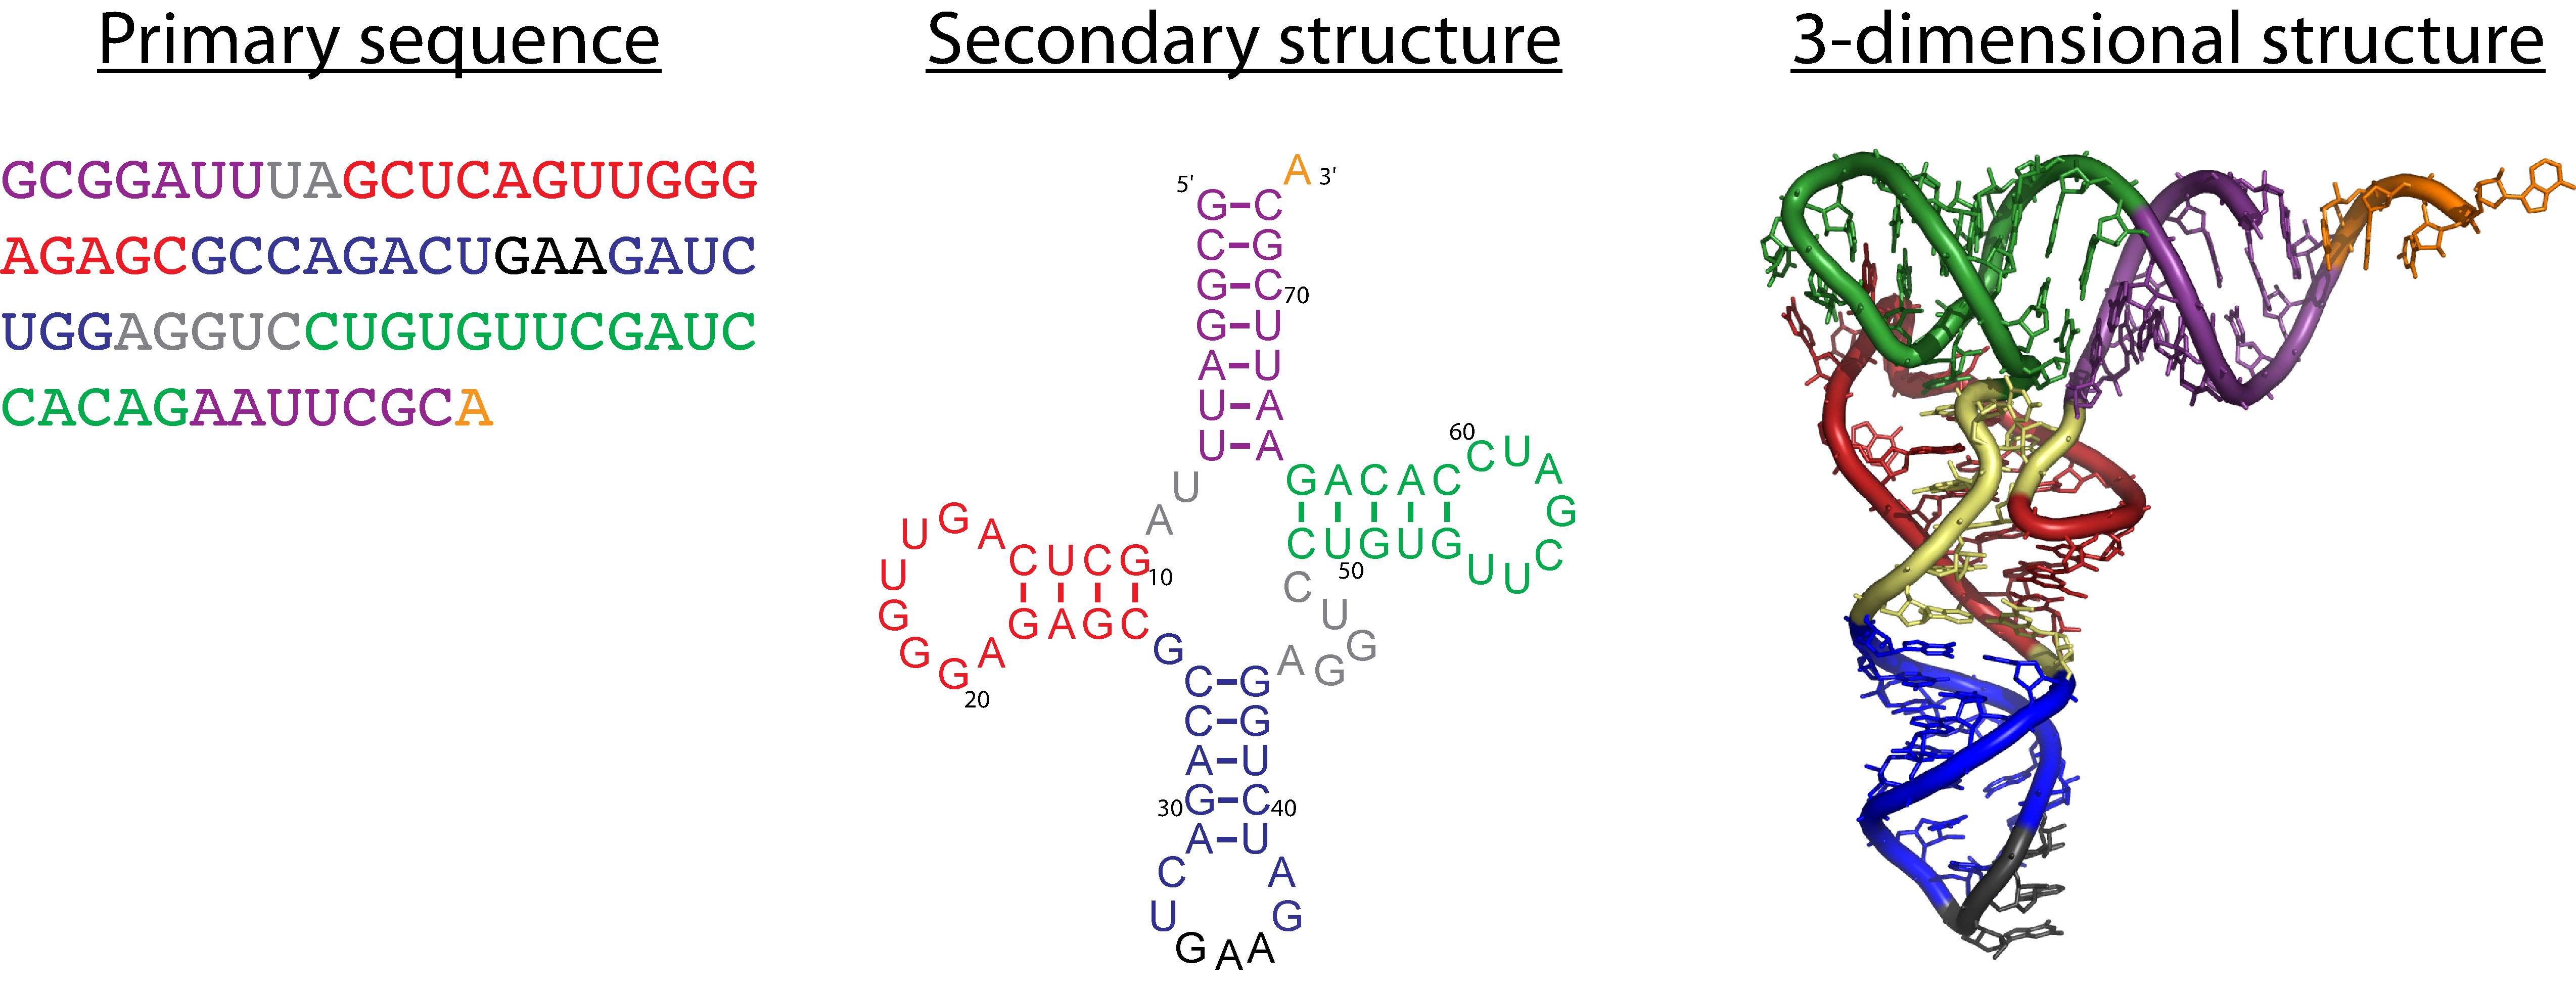
\includegraphics[width=10.5in]{figs/trna-123}
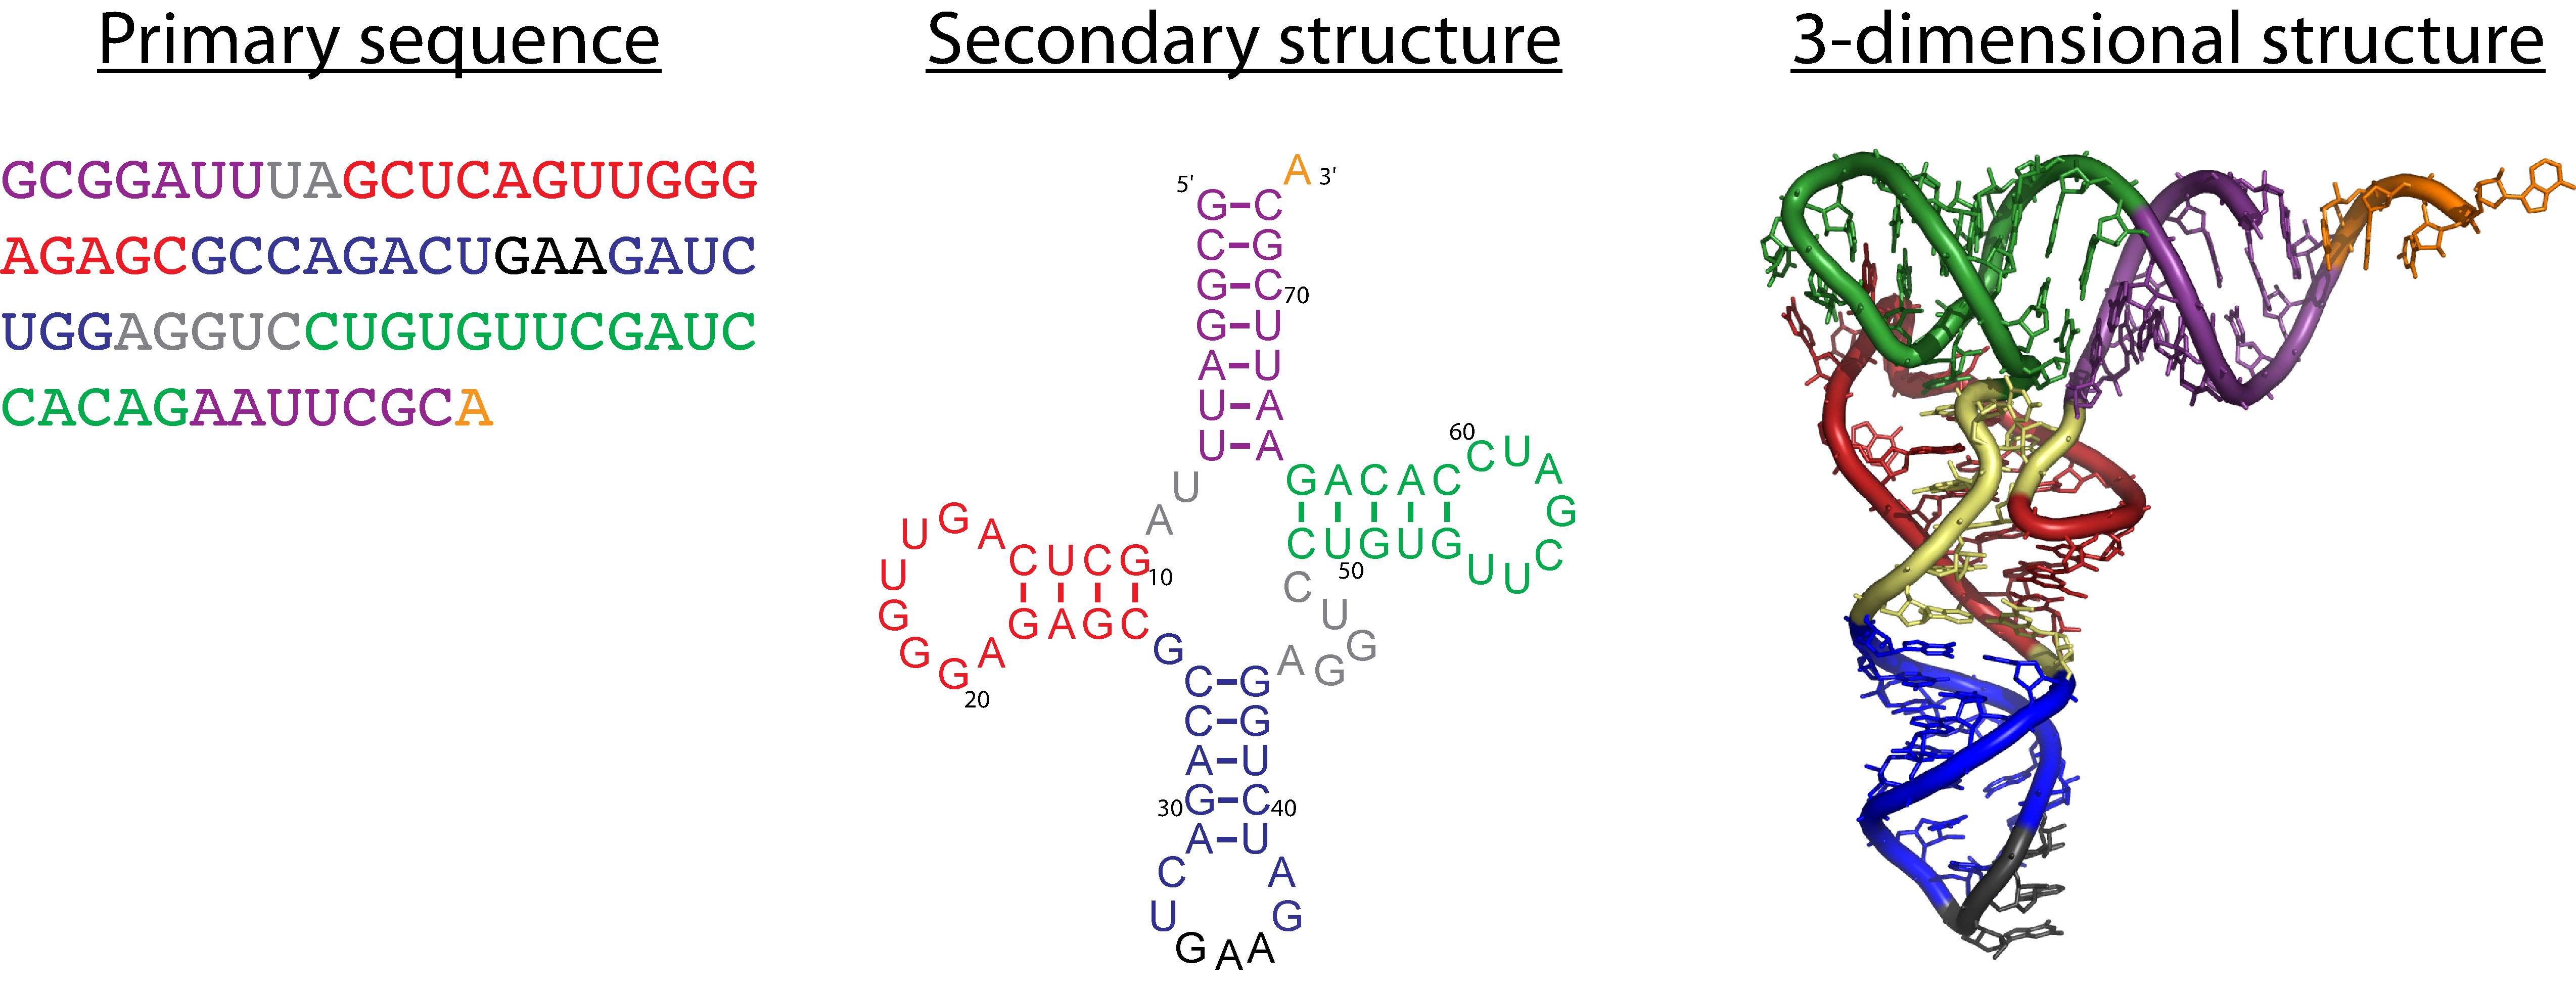
\includegraphics[width=9in]{figs/trna-123}

\end{center}

\vfill

\end{slide}
%%%%%%%%%%%%%%%%%%%%%%%%%%%%%%%%%%%%%%%%%%%%%%%%%%%%%%%%%%%%%%
\begin{slide}
\begin{center}
{\bf Many functional RNAs adopt a conserved 3-dimensional 
  structure}

\medskip

Three representations of a transfer RNA:

%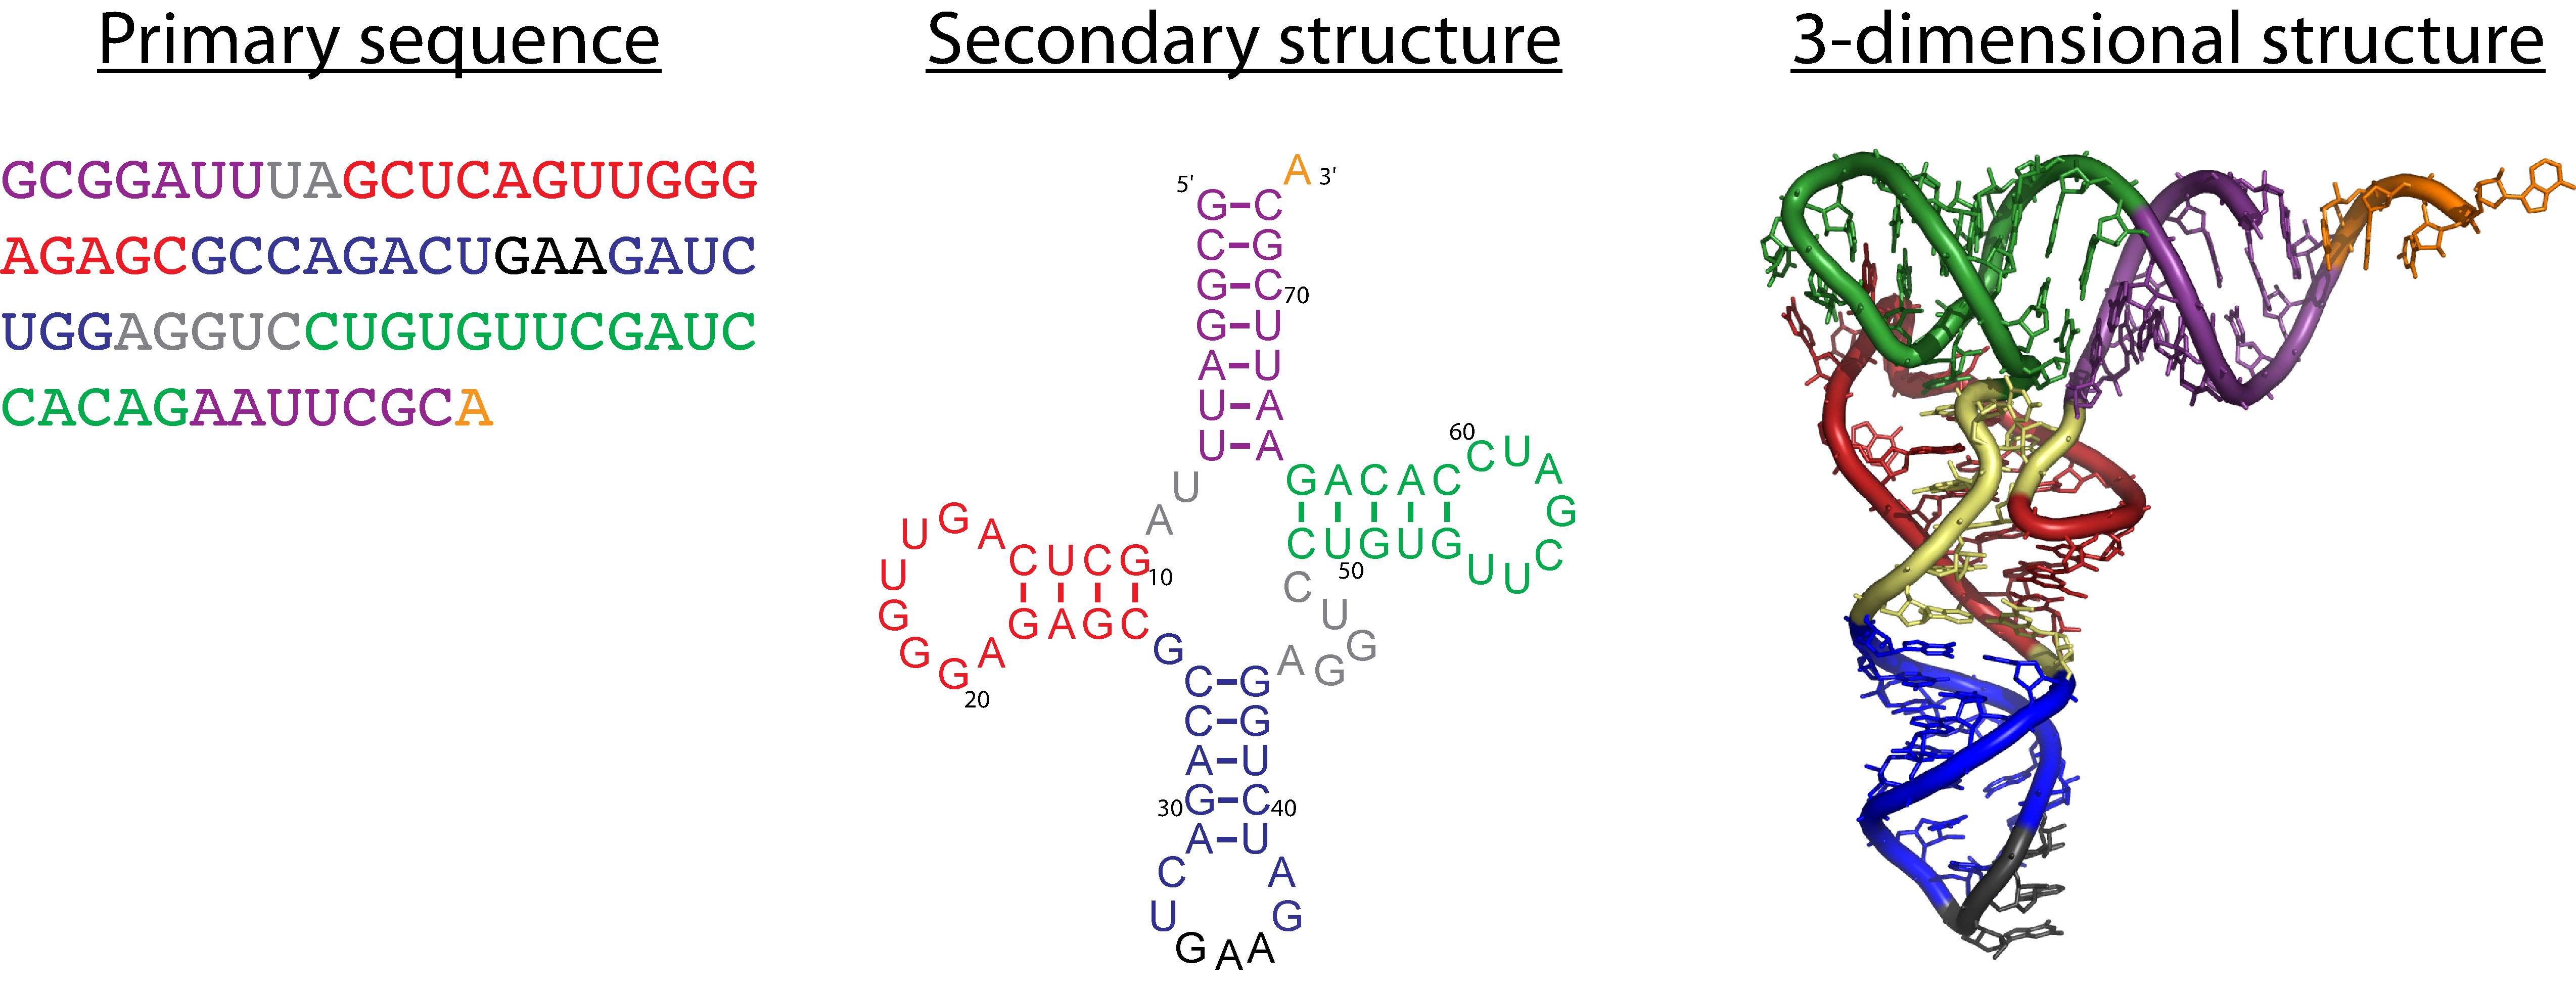
\includegraphics[width=10.5in]{figs/trna-123}
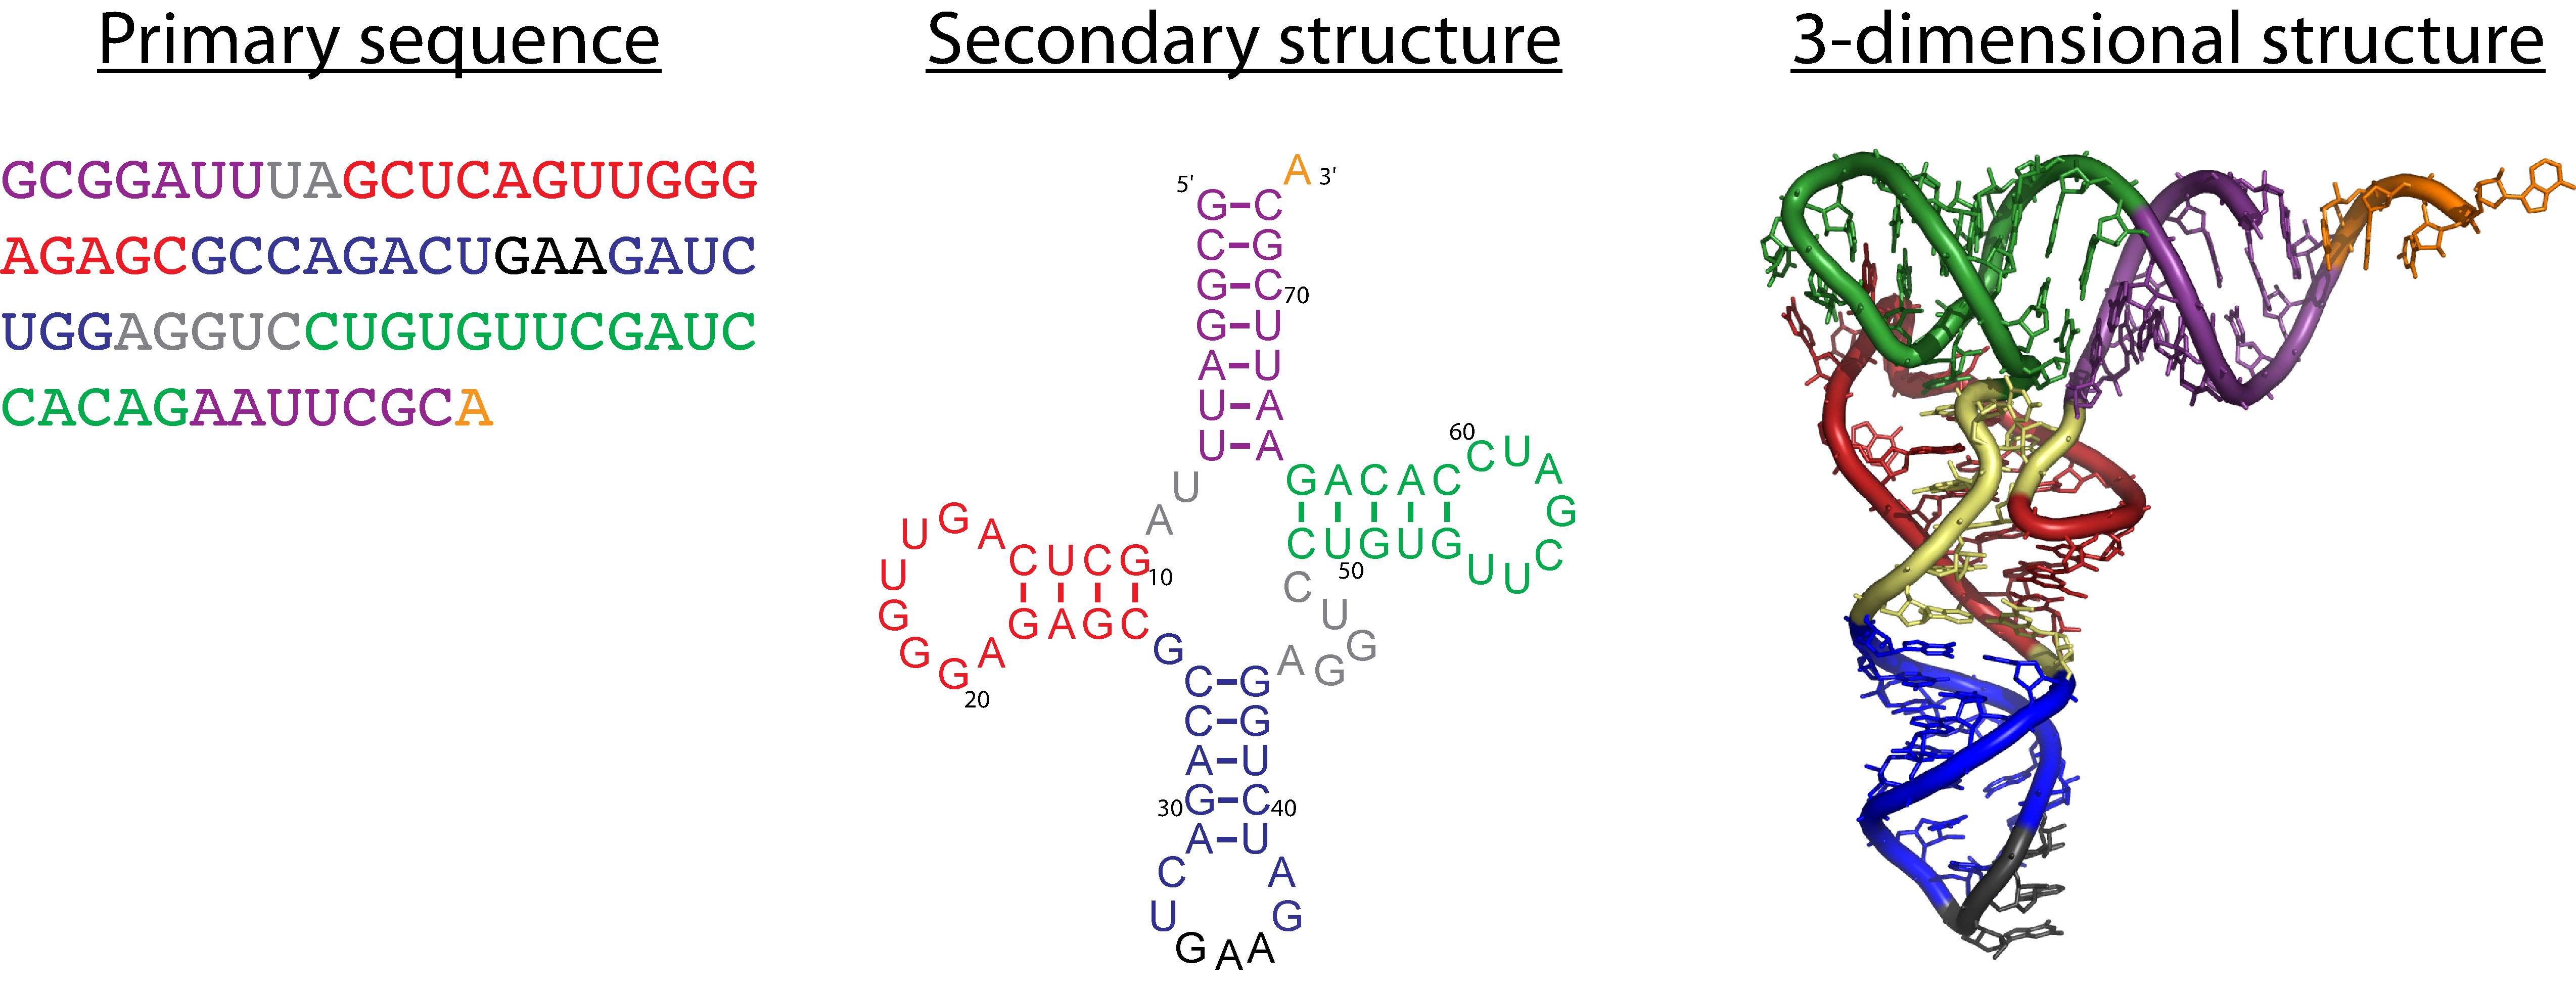
\includegraphics[width=9in]{figs/trna-123}
\end{center}

\begin{itemize}
\item
  BLAST: given a single sequence, search genomes for similar sequences.
\item
  BLAST cannot take advantage of:
\begin{itemize}
  \item secondary structure
  \item sequence conservation, which varies across the gene
\end{itemize}
\end{itemize}

\vfill

\end{slide}
%%%%%%%%%%%%%%%%%%%%%%%%%%%%%%%%%%%%%%%%%%%%%%%%%%%%%%%%%%%%%
\begin{slide}
\begin{center}
%\textbf{Comparative analysis of sequence families}: \\
\textbf{Sequence conservation provides \\ information for homology searches}

\medskip
Conservation levels vary across alignment columns.

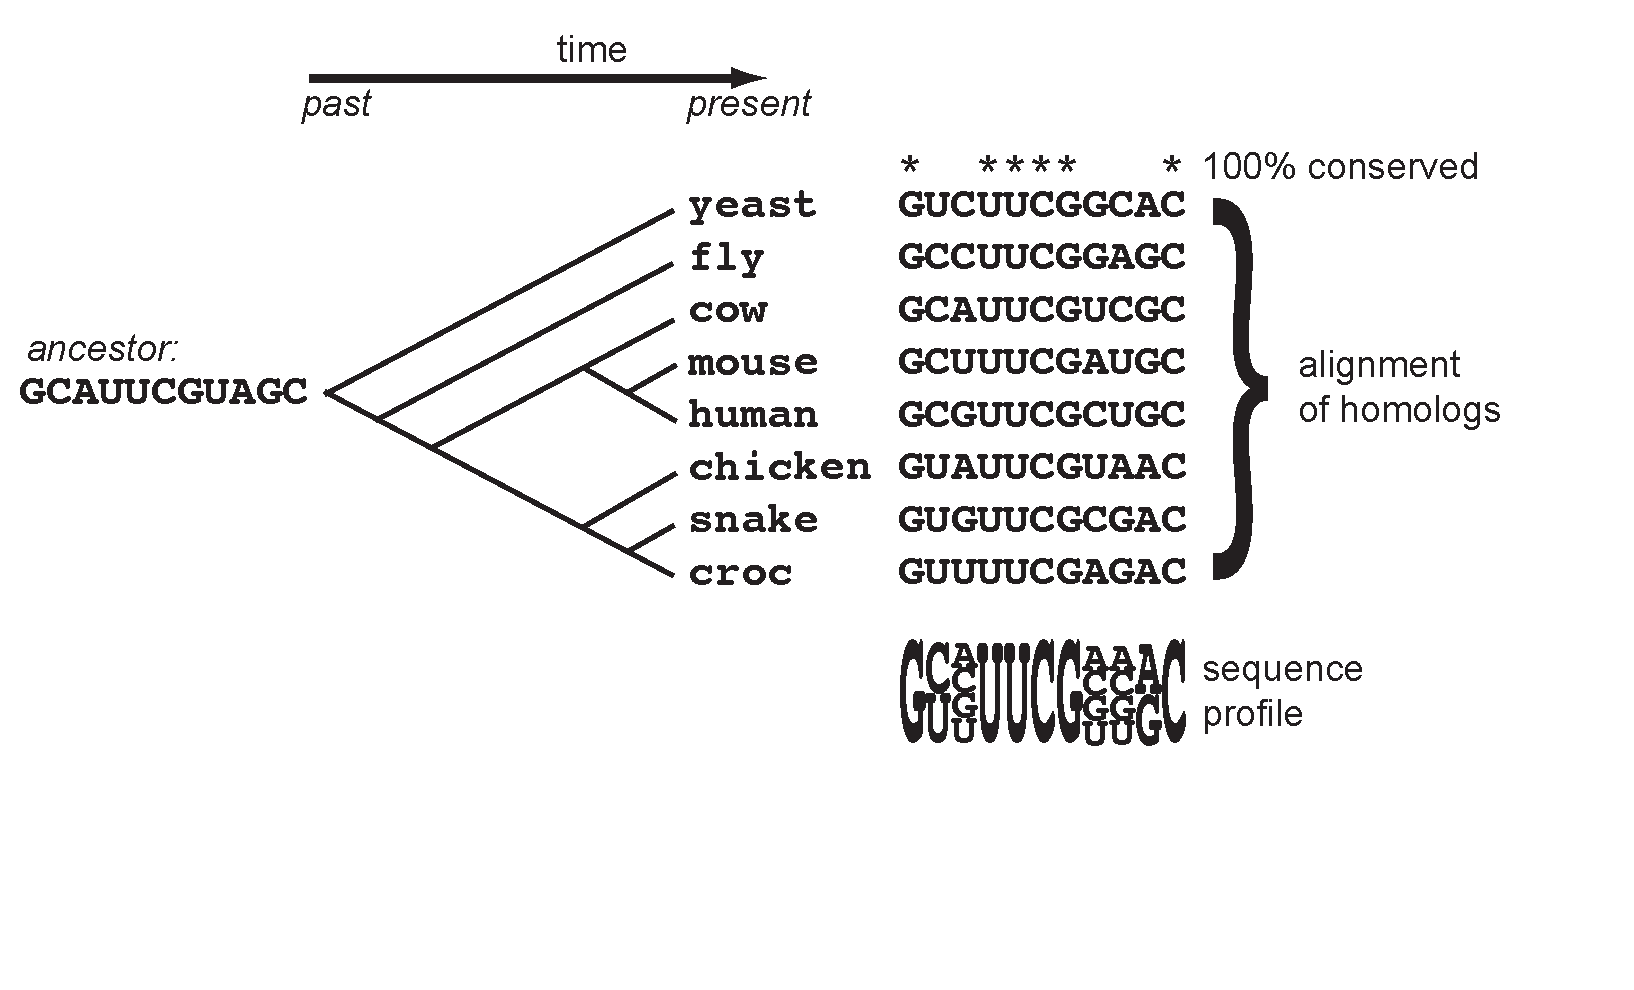
\includegraphics[width=10in]{figs/seqstructprofiles-seq1}
\end{center}

\vfill
\end{slide}
%%%%%%%%%%%%%%%%%%%%%%%%%%%%%%%%%%%%%%%%%%%%%%%%%%%%%%%%%%%%%%%%%%%%%%
\begin{slide}
\begin{center}
\textbf{Structure conservation provides additional information}
\medskip

Base-paired positions covary \\ to maintain Watson-Crick complementarity.

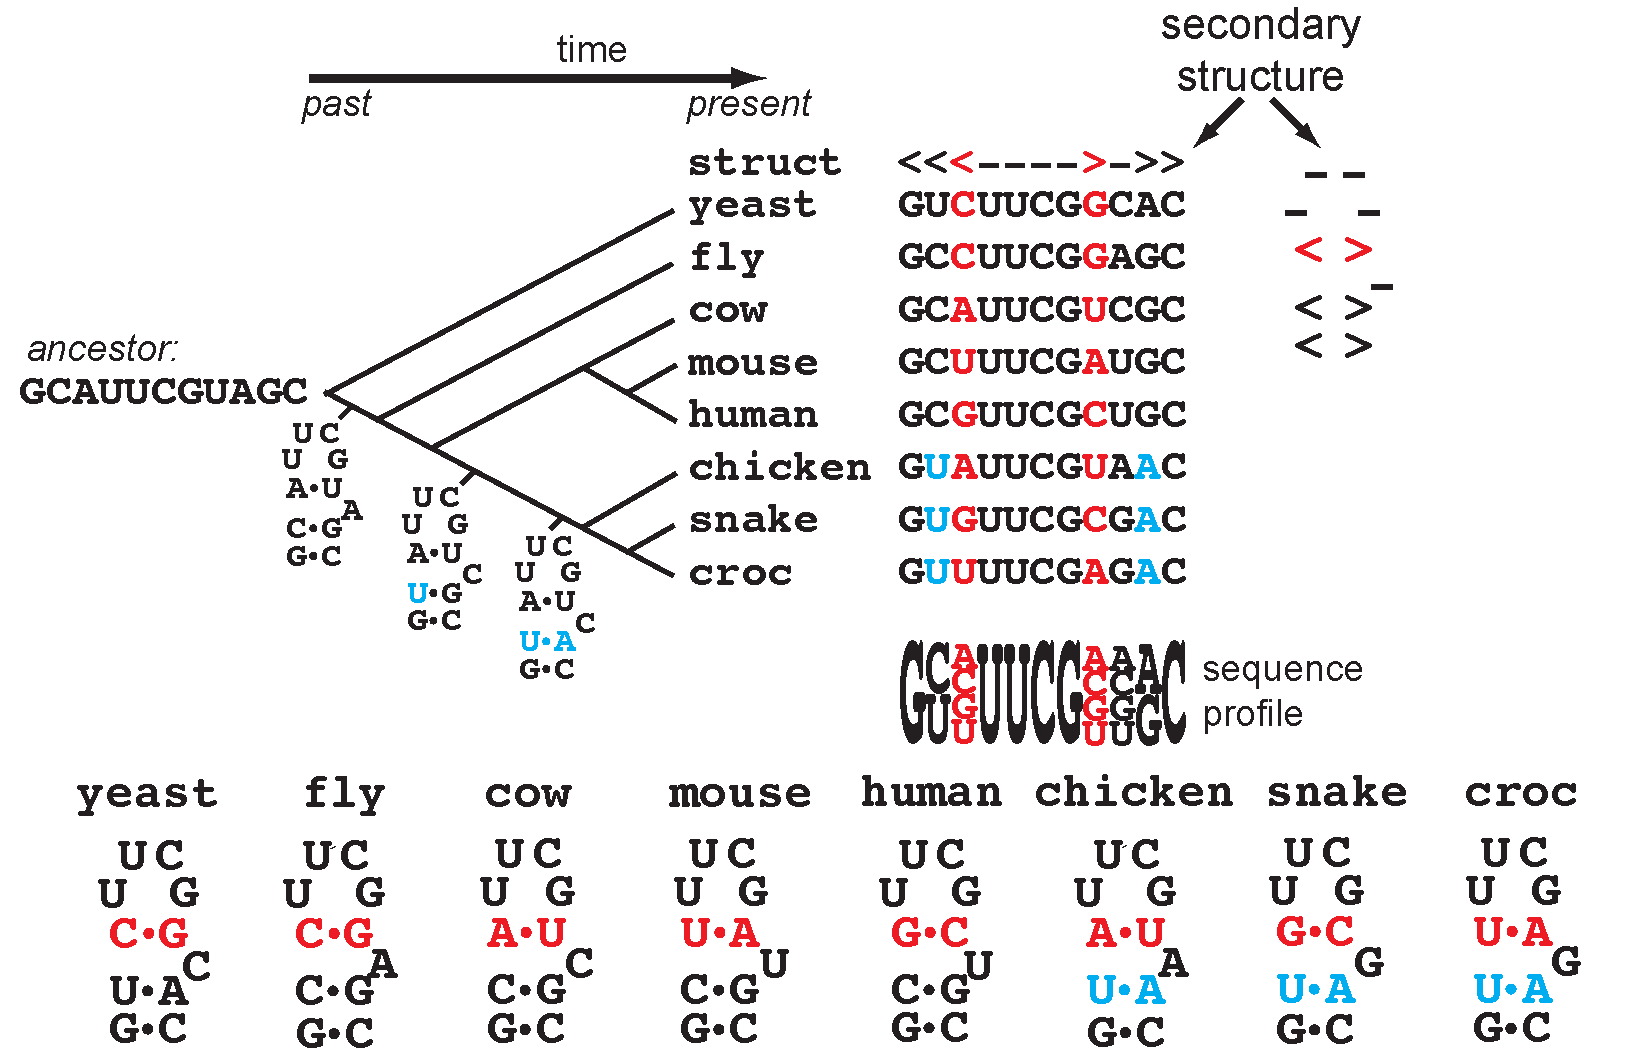
\includegraphics[width=10in]{figs/seqstructprofiles-struct2}
\end{center}

\vfill
\end{slide}
%%%%%%%%%%%%%%%%%%%%%%%%%%%%%%%%%%%%%%%%%%%%%%%%%%%%%%%%%%%%%%%%%%%%%%%%%%
\begin{slide}
\begin{center}
\textbf{Amount of information in a profile can be measured in bits}
\medskip

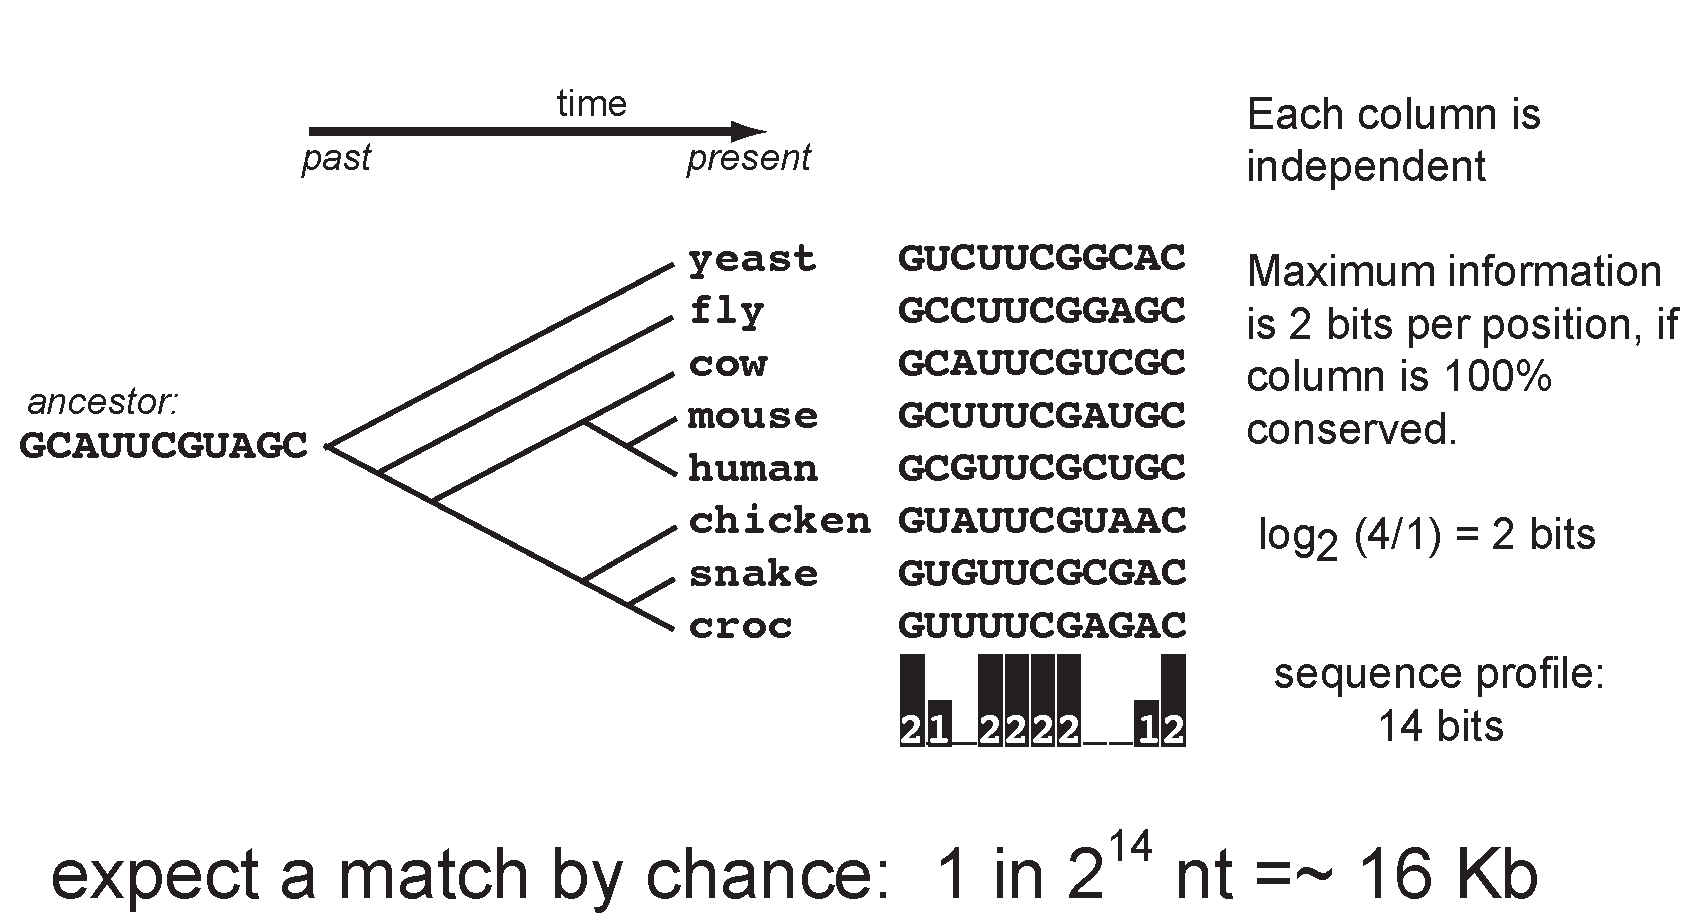
\includegraphics[width=9in]{figs/seqstructprofiles-2014-seqinfo}
\end{center}

\vfill
\end{slide}
%%%%%%%%%%%%%%%%%%%%%%%%%%%%%%%%%%%%%%%%%%%%%%%%%%%%%%%%%%%%%%%%%%%%%%%%%%
\begin{slide}
\begin{center}
\textbf{Structure contributes additional information from covariation}
\medskip

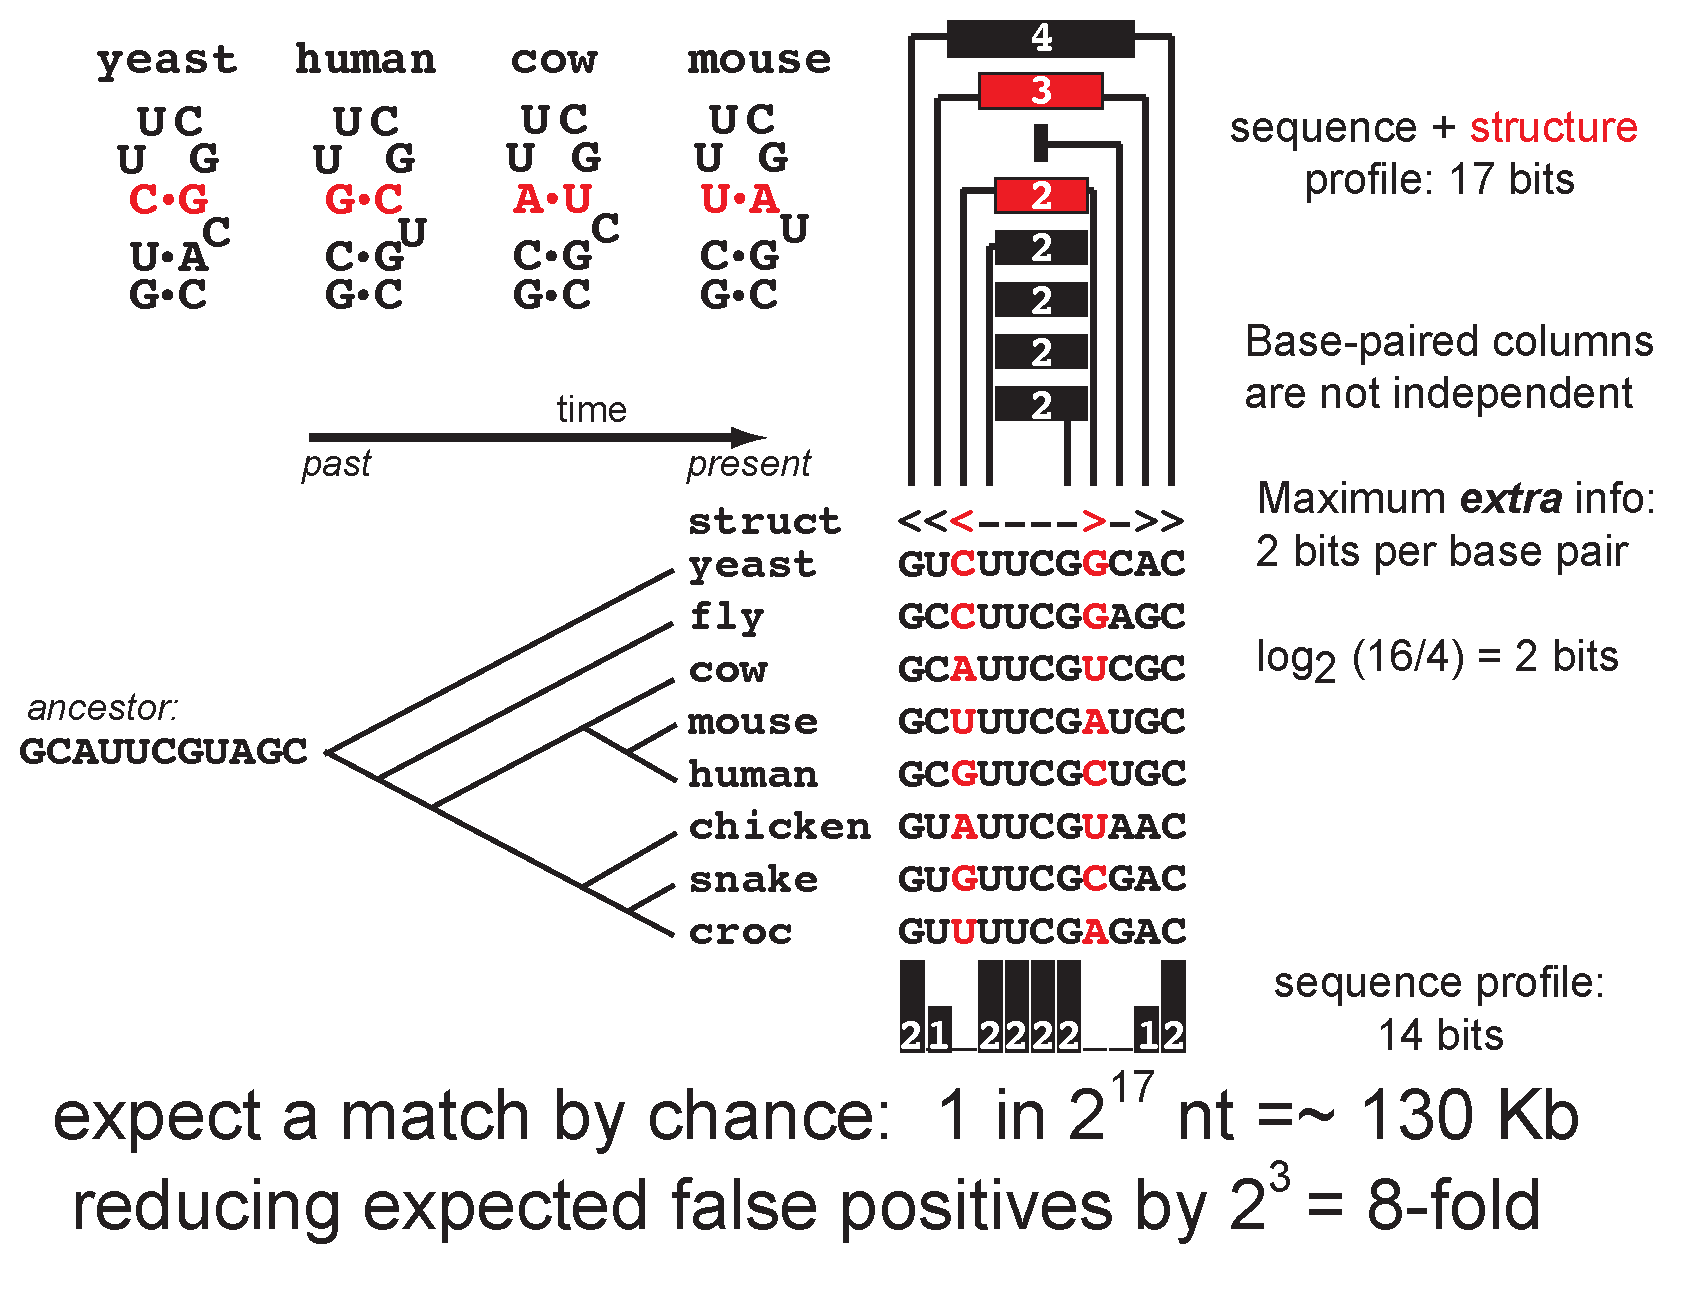
\includegraphics[width=9in]{figs/seqstructprofiles-2014-structinfo}
\end{center}

\vfill
\end{slide}
%%%%%%%%%%%%%%%%%%%%%%%%%%%%%%%%%%%%%%%%%%%%%%%%%%%%%%%%%%%%%%%%%%%%%%%%%%
\begin{slide}
\begin{center}
\textbf{Levels of sequence and structure conservation in RNA families}
\end{center}
\medskip

\begin{center}
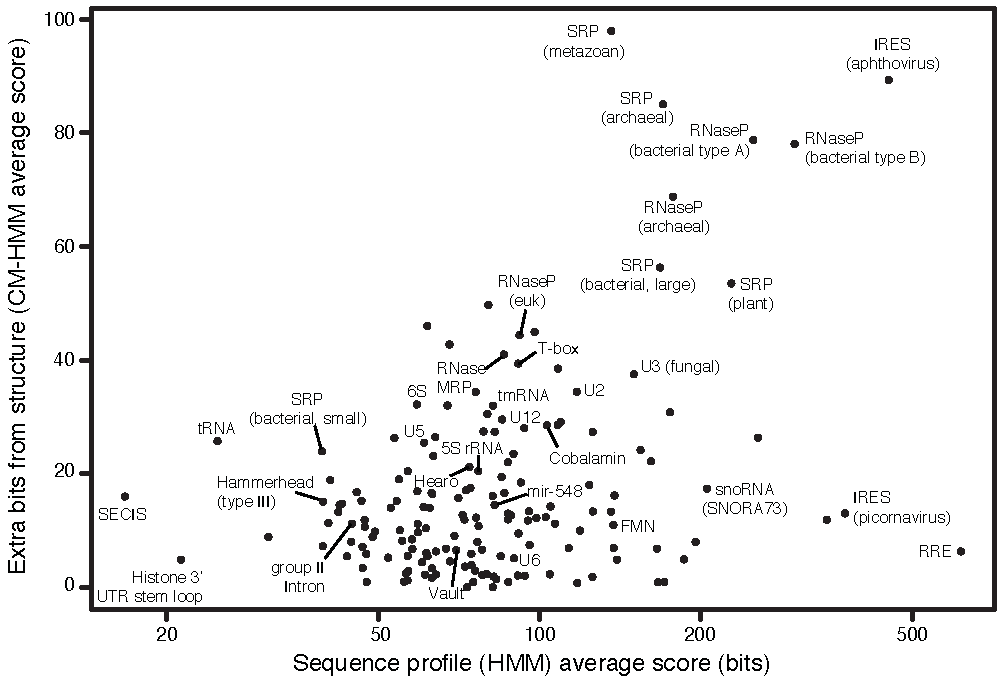
\includegraphics[height=6.5in]{figs/avgscores-rfam11}
\end{center}

\vfill

\end{slide}
%%%%%%%%%%%%%%%%%%%%%%%%%%%%%%%%%%%%%%%%%%%%%%%%%%%%%%%%%%%%%%%%%%%
\begin{slide}
\begin{center}
%\textbf{profile HMMs and covariance models}
\textbf{Eddy lab software for profile probabilistic models } (since 1994)
\end{center}
\medskip

\begin{center}
\small
\begin{tabular}{r|cc} 
%             &         & sequence \\
%             & sequence& and structure \\
%             & profiles& profiles \\ \hline
             & sequence & sequence and \\
             & profiles & structure profiles \\ \hline
  \\
  models     & profile HMMs     & {\color{red} covariance models (CMs)} \\ 
  \\
  software   & {\sc HMMER}      & {\sc Infernal} \\ 
  \\
  main use   & proteins,         & structural RNAs \\ 
             & repetitive DNA elements &  \\
  \\
  databases  & {\sc Pfam} and \sc{Dfam}       & {\sc Rfam} \\
             & (14831 and 1132 entries) & (2450 families) \\
  \\
%  primary sequence & yes & yes \\
%  \\
%  secondary structure & no & yes \\
%  \\
%  algorithms & Viterbi, Forward & CYK, Inside \\
%%             & Forward & Inside \\
%             &         & \\
%  complexity & $O(LN)$ & $O(LN^{2} log N)$ \\
%  \\
  performance& faster but    & slower but    \\
  for RNAs   & less accurate & more accurate \\
\end{tabular}

%\hspace{1.2in}
\includegraphics[height=2in]{figs/hmmer_logo}\hspace{1.05in}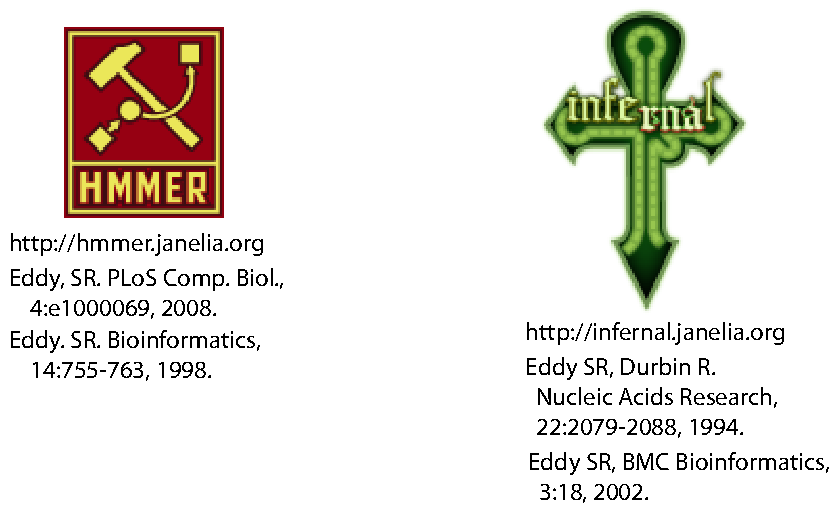
\includegraphics[height=2.6in]{figs/infernal_logo}
\hspace{1.8in}
\includegraphics[height=2.7in]{figs/hmmer-infernal-refs-2014}

\end{center}

\vfill

\end{slide}
%%%%%%%%%%%%%%%%%%%%%%%%%%%%%%%%%%%%%%%%%%%%%%%%%%%%%%%%%%%%%%%
\begin{slide}
\begin{center}
\textbf{Is the added complexity worth it? \\
  RMARK: a challenging \underline{internal} RNA homology search
  benchmark}

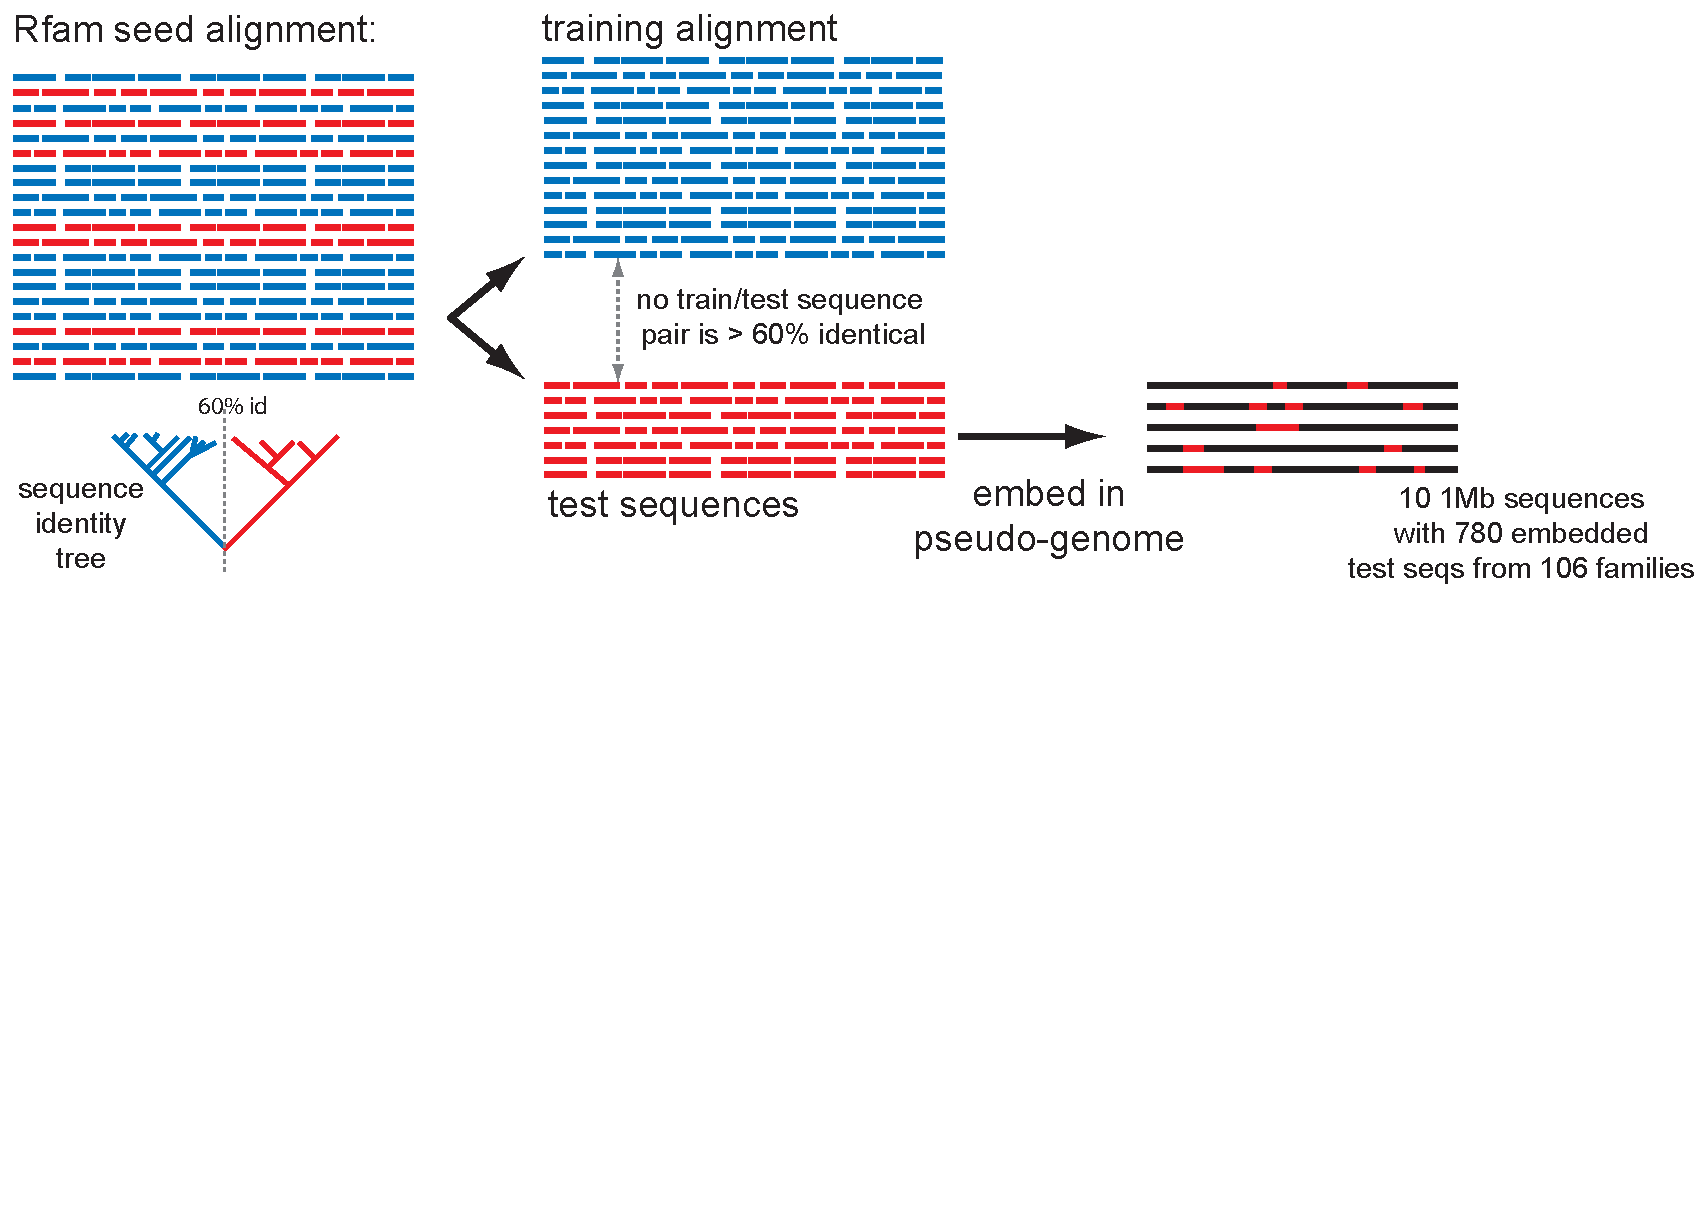
\includegraphics[width=10in]{figs/rmark-tree-1}
\end{center}

\vfill
\end{slide}
%%%%%%%%%%%%%%%%%%%%%%%%%%%%%%%%%%%%%%%%%%%%%%%%%%%%%%%%%%%%%%%%%%%%%%
\begin{slide}
\begin{center}
\textbf{Is the added complexity worth it? \\
  RMARK: a challenging \underline{internal} RNA homology search
  benchmark}

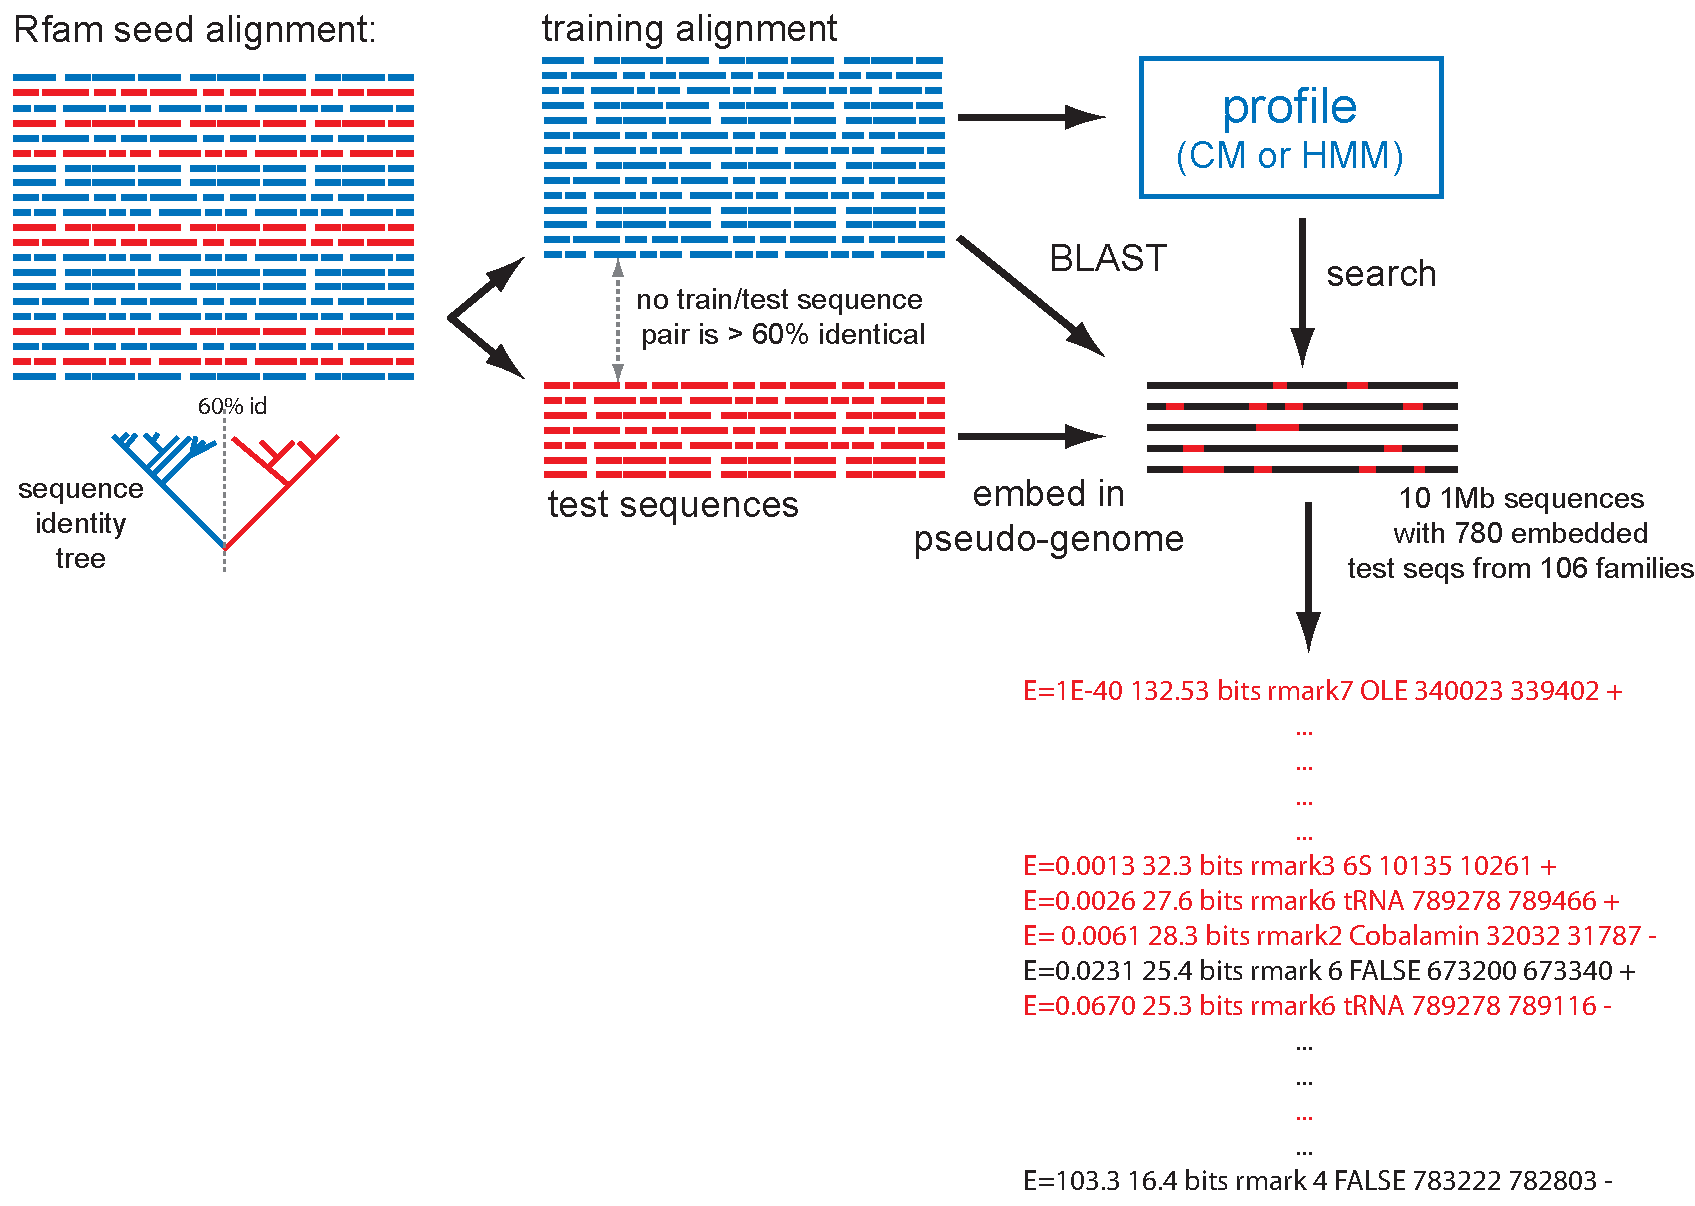
\includegraphics[width=10in]{figs/rmark-tree-2}
\end{center}

\vfill
\end{slide}
%%%%%%%%%%%%%%%%%%%%%%%%%%%%%%%%%%%%%%%%%%%%%%%%%%%%%%%%%%%%%%%%%%%%%%
\begin{slide}
\begin{center}

\textbf{Infernal outperforms primary-sequence based methods on our
  benchmark (and others\footnote{Freyhult EK, Bollback JP, Gardner
    PP. Genome Res. 2007 17: 117-125.}, not shown)}

\end{center}
\medskip

\center{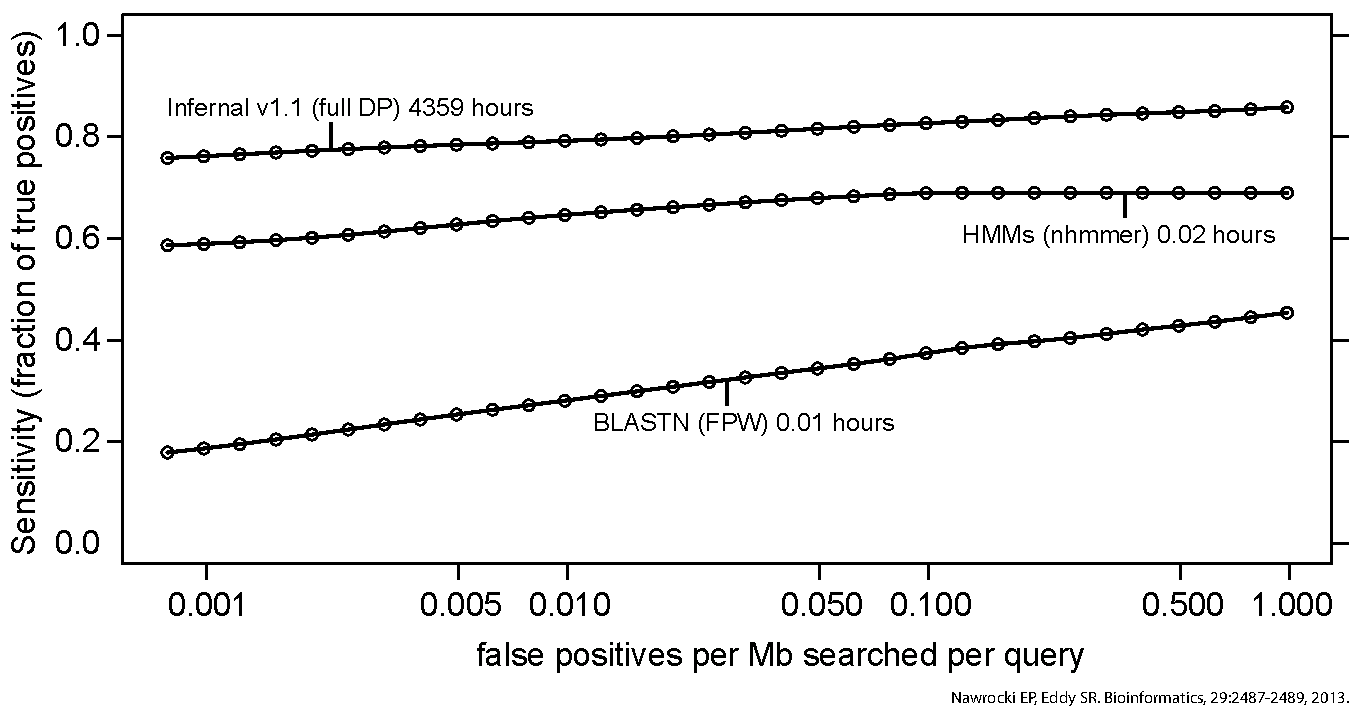
\includegraphics[width=10in]{figs/roc-talk-rcb-2014-1}}

\vfill 
\end{slide}
%%%%%%%%%%%%%%%%%%%%%%%%%%%%%%%%%%%%%%%%%%%%%%%%%%%%%%%%%%%%%%%%%%%%%%
\begin{slide}
\begin{center}
\large
\textbf{Filter target database using profile HMMs\footnote{Weinberg, Ruzzo, RECOMB, 243-251, 2004}}
\end{center}

\center{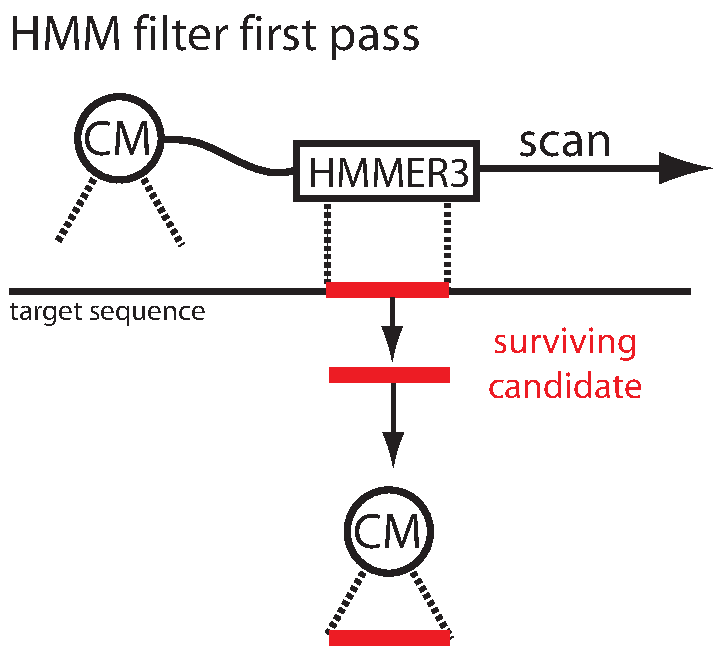
\includegraphics[height=4in]{figs/filter-2014-1}}

\vfill
\end{slide}
%%%%%%%%%%%%%%%%%%%%%%%%%%%%%%%%%%%%%%%%%%%%%%%%%%%%%%%%%%%%%%%%%%%%%%%%%%
\begin{slide}
\begin{center}
\large
\textbf{Filter target database using profile HMMs\footnote{Weinberg, Ruzzo, RECOMB, 243-251, 2004}}
\end{center}

\center{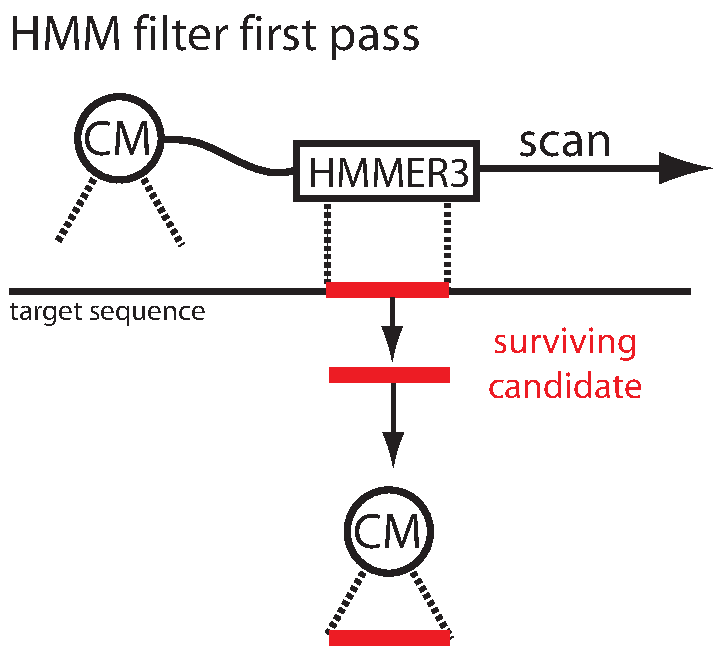
\includegraphics[height=4in]{figs/filter-2014-1}}

\begin{itemize}
\item Even if we filter out 99\% of the database (for up to 100X
  acceleration), searches will still be too slow.
\item CM step needs to be accelerated. 
\end{itemize}

\vfill
\end{slide}
%%%%%%%%%%%%%%%%%%%%%%%%%%%%%%%%%%%%%%%%%%%%%%%%%%%%%%%%%%%%%%%%%%%%%%%%%%
\begin{slide}
\begin{center}

\textbf{Accelerating CM alignment step 1: \\ align sequence with HMM}

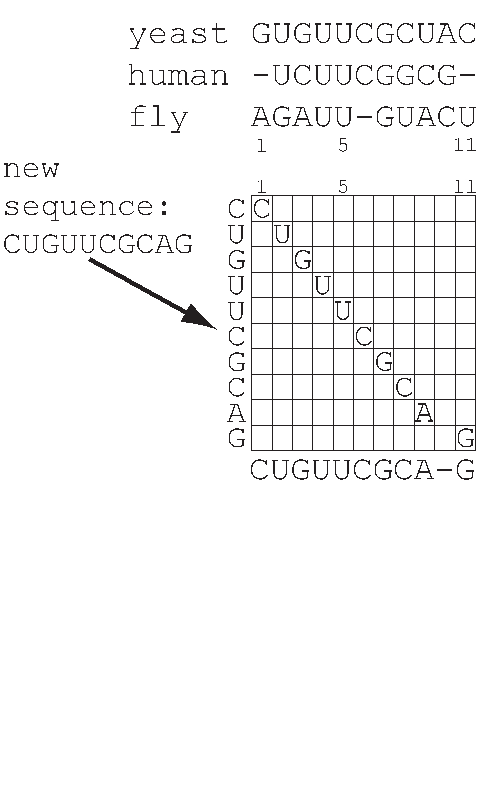
\includegraphics[height=6in]{figs/hmm_alignment2_layer2}
\end{center}

\vfill
\end{slide}
%%%%%%%%%%%%%%%%%%%%%%%%%%%%%%%%%%%%%
%%%%%%%%%%%%%%%%%%%%%%%%%%%%%%%%%%%%%%%%%%%%%%%%%%%%%%%%%%%%%%%%%%%%%%%%%%
\begin{slide}
\begin{center}

\textbf{Accelerating CM alignment step 2: \\ HMM posterior decoding to
  get confidence estimates}

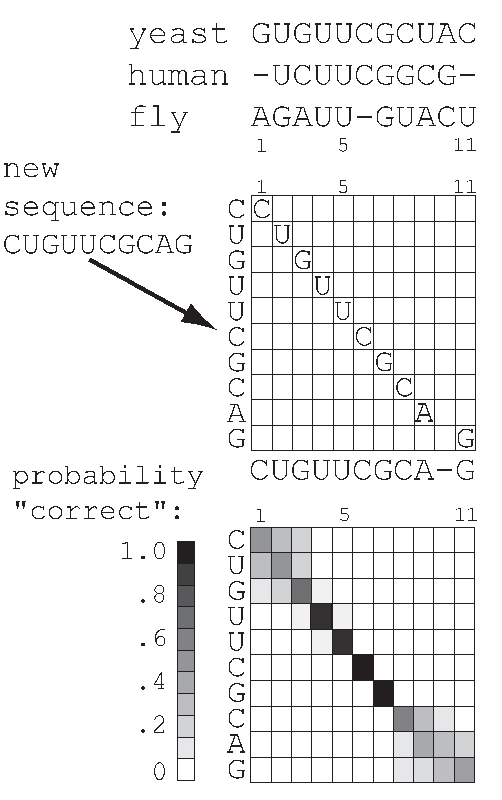
\includegraphics[height=6in]{figs/hmm_alignment2_layer3}
\end{center}

\vfill
\end{slide}
%%%%%%%%%%%%%%%%%%%%%%%%%%%%%%%%%%%%%
\begin{slide}
\begin{center}

\textbf{Accelerating CM alignment step 3: \\ use HMM alignment
  confidence to constrain CM alignment\footnote{M. P. Brown. Proc. Int. Conf. ISMB, 8:57–66, 2000.}}
\end{center}
\medskip
\small
%\begin{itemize}
%\item
%\textbf{main idea:} eliminate potential alignments the HMM tells us are very improbable
%\end{itemize}
\begin{center}
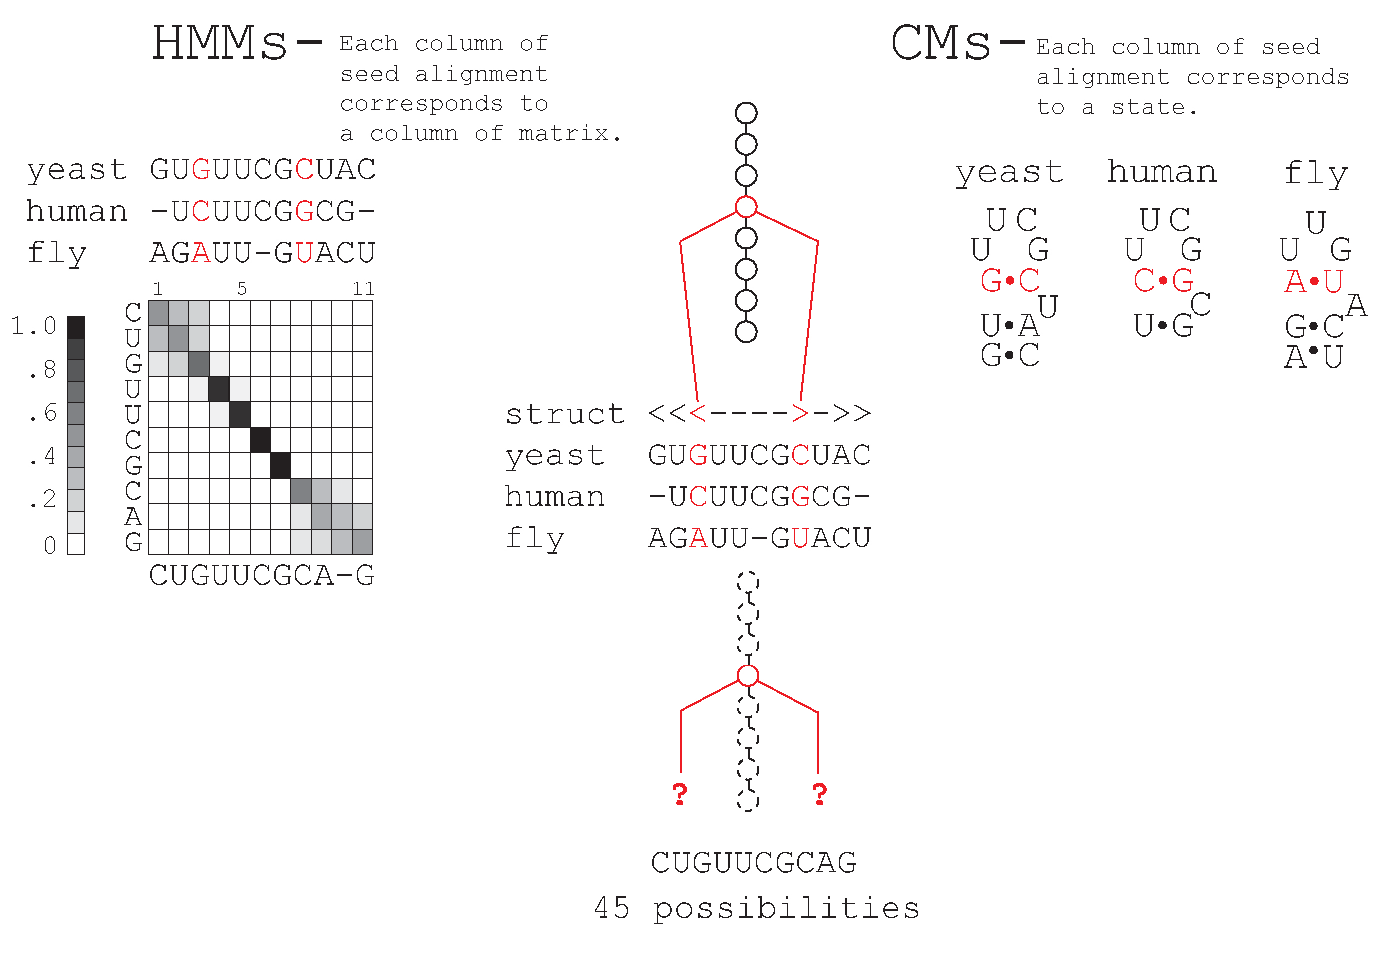
\includegraphics[width=8in]{figs/post_hmm_to_cm_map2_layer14}
\end{center}
\vfill
\end{slide}
%%%%%%%%%%%%%%%%%%%%%%%%%%%%%%%%%%%%%%%%%%%%%%%%%%%%%%%%%%%%%%%%%%%%%%
\begin{slide}
\begin{center}

\textbf{Accelerating CM alignment step 3: \\ use HMM alignment
  confidence to constrain CM alignment\footnote{M. P. Brown. Proc. Int. Conf. ISMB, 8:57–66, 2000.}}
\end{center}
\medskip
\small
%\begin{itemize}
%\item
%\textbf{main idea:} eliminate potential alignments the HMM tells us are very improbable
%\end{itemize}
\begin{center}
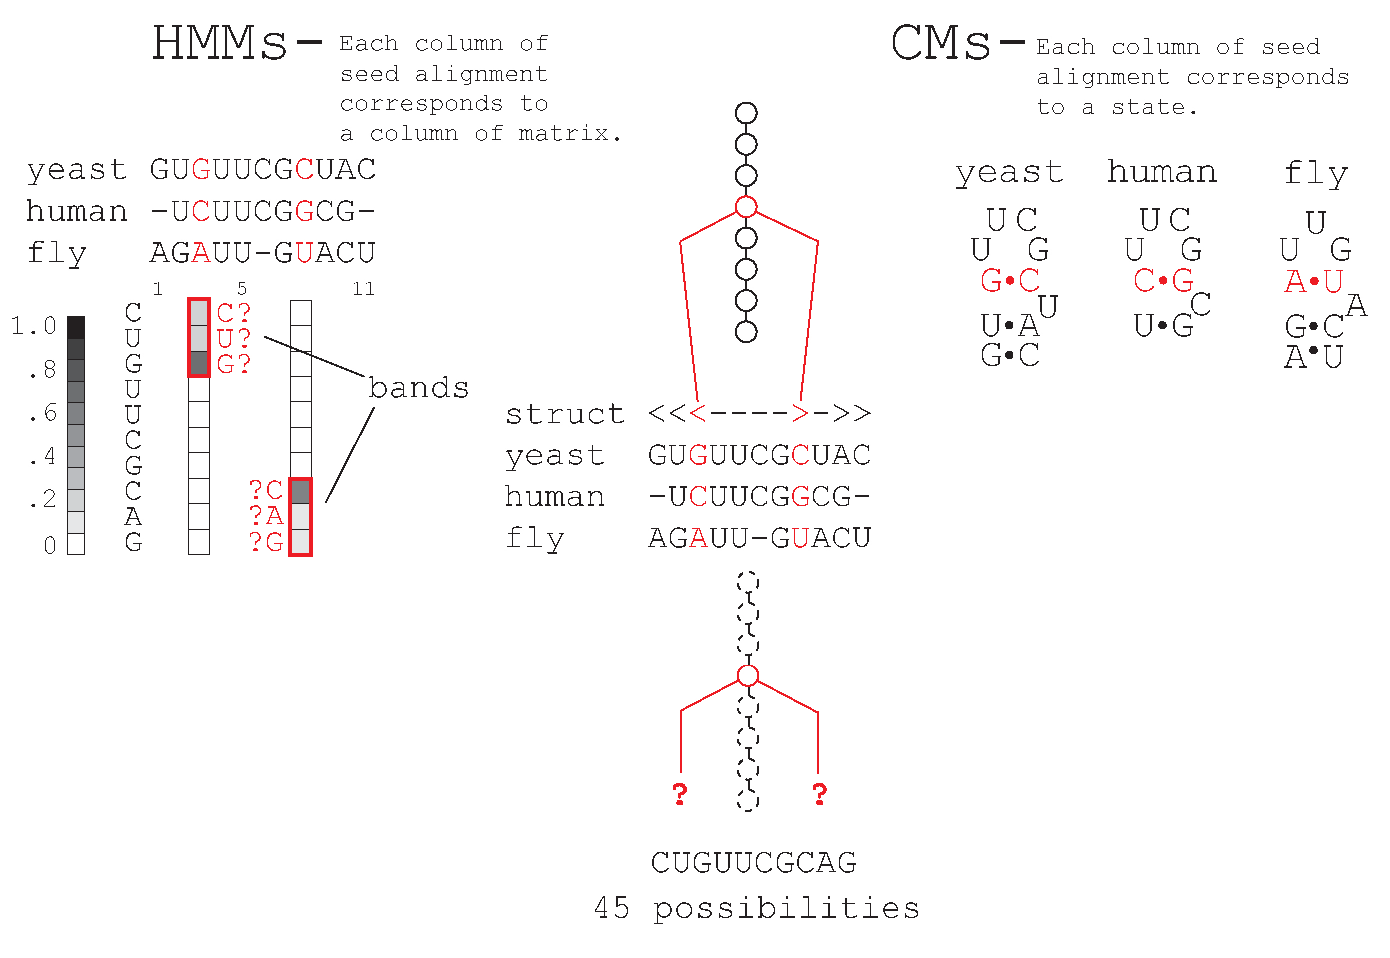
\includegraphics[width=8in]{figs/post_hmm_to_cm_map2_layer15}
\end{center}
\vfill
\end{slide}
%%%%%%%%%%%%%%%%%%%%%%%%%%%%%%%%%%%%%%%%%%%%%%%%%%%%%%%%%%%%%%%%%%%%%%%%%%
\begin{slide}
\begin{center}

\textbf{Accelerating CM alignment step 3: \\ use HMM alignment
  confidence to constrain CM alignment\footnote{M. P. Brown. Proc. Int. Conf. ISMB, 8:57–66, 2000.}}
\end{center}
\medskip
\small
%\begin{itemize}
%\item
%\textbf{main idea:} eliminate potential alignments the HMM tells us are very improbable
%\end{itemize}
\begin{center}
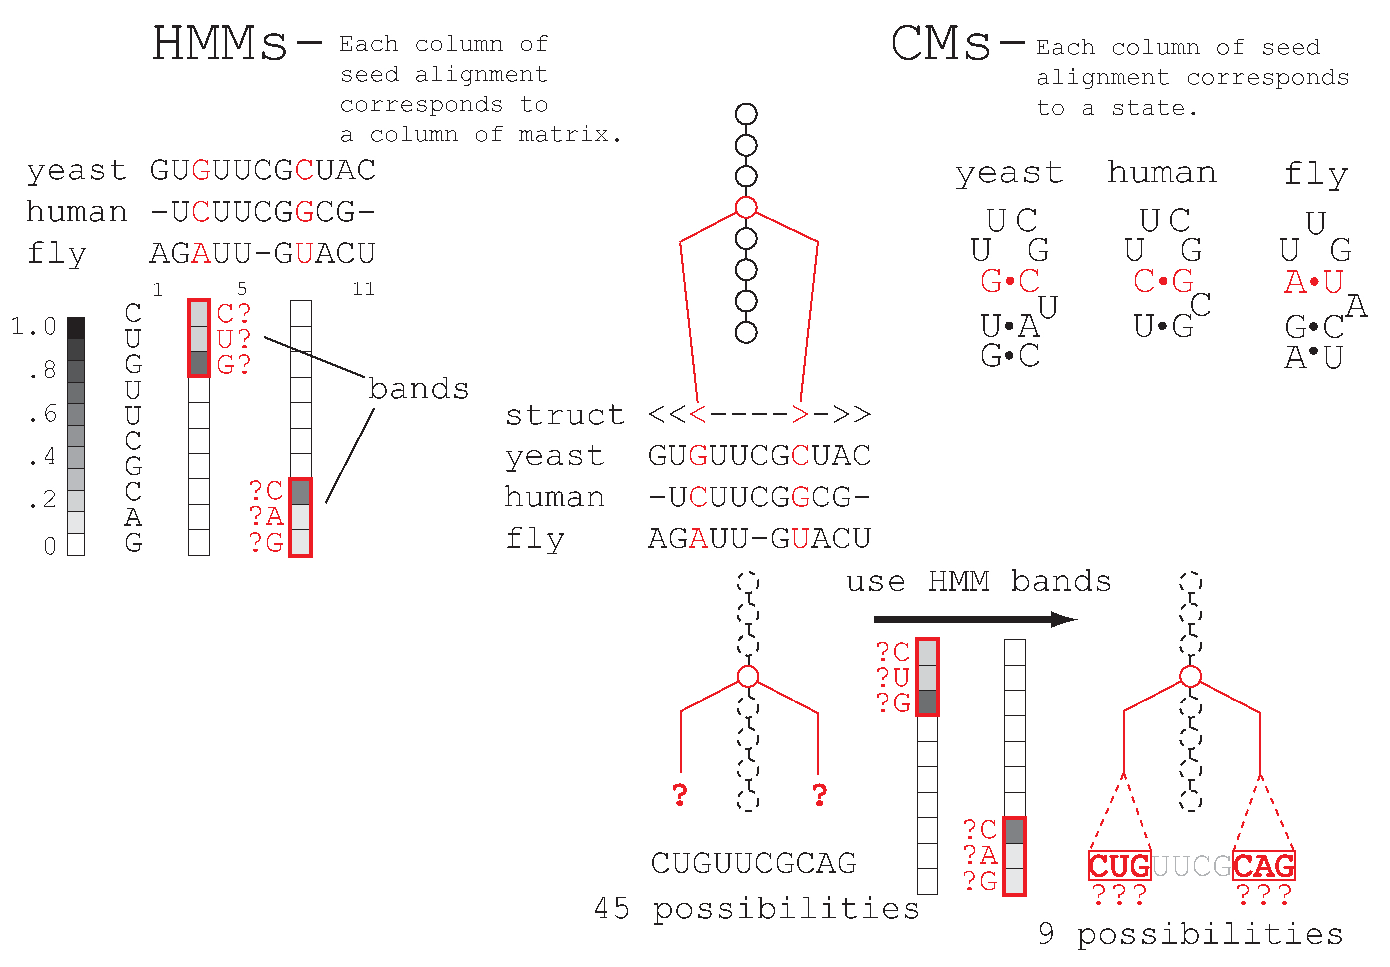
\includegraphics[width=8in]{figs/post_hmm_to_cm_map2_layer16}
\end{center}
\vfill
\end{slide}
%%%%%%%%%%%%%%%%%%%%%%%%%%%%%%%%%%%%%%%%%%%%%%%%%%%%%%%%%%%%%%%%%%%%%%
\begin{slide}
\begin{center}
\large
\textbf{Use HMMs as filters and to constrain CM alignment}
\end{center}

\center{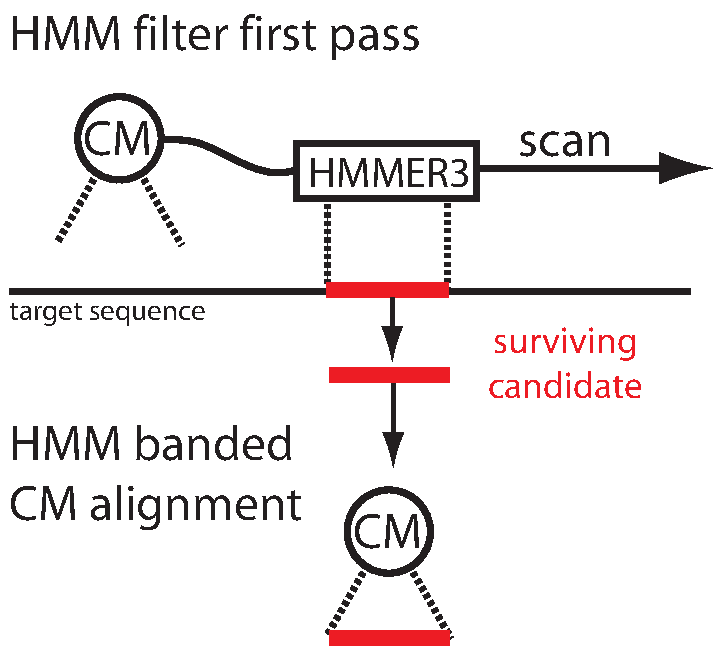
\includegraphics[height=5in]{figs/filter-2014-2}}

\vfill
\end{slide}
%%%%%%%%%%%%%%%%%%%%%%%%%%%%%%%%%%%%%%%%%%%%%%%%%%%%%%%%%%%%%%%%%%%%%%%%%%
\begin{slide}
\begin{center}

\textbf{HMM-based acceleration makes Infernal 10,000 times faster}

\end{center}
\medskip

\center{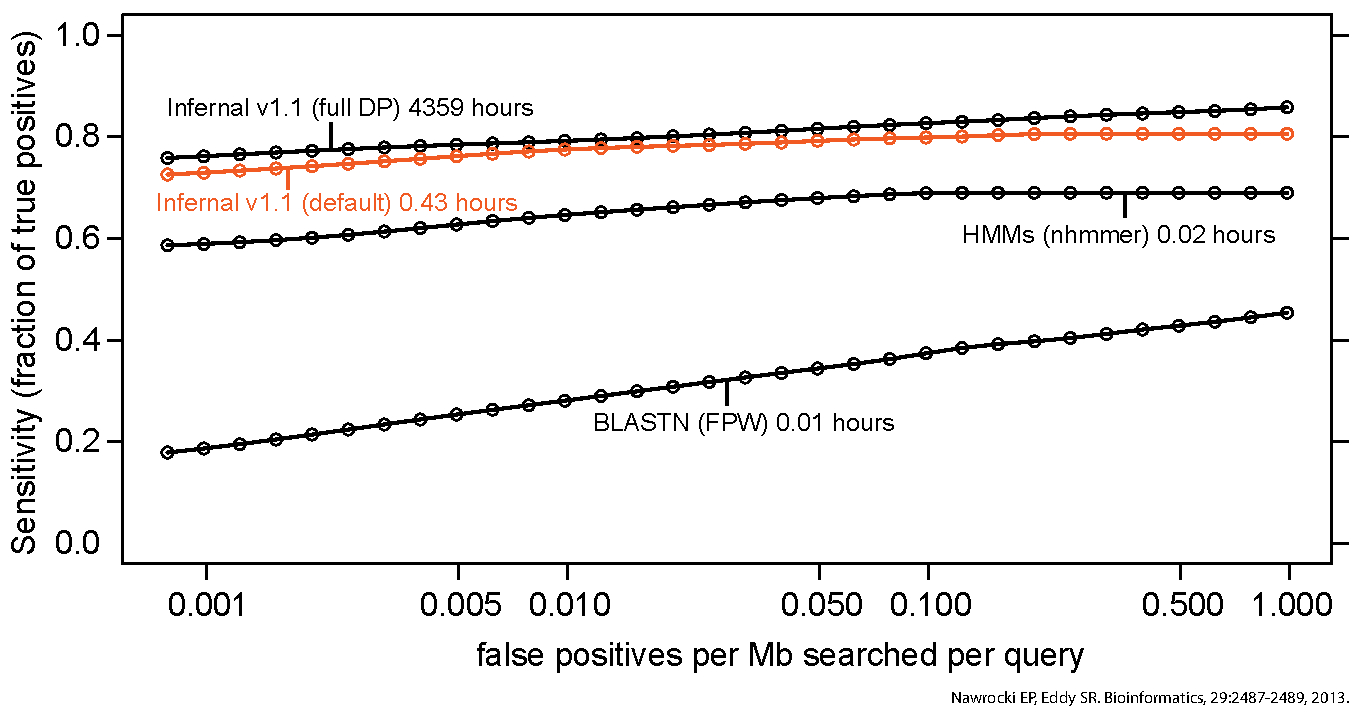
\includegraphics[width=10in]{figs/roc-talk-rcb-2014-2}}

\vfill 
\end{slide}


%%%%%%%%%%%%%%%%%%%%%%%%%%%%%%%%%%%%%%%%%%%%%%%%%%%%%%%%%%%%%%%%%%%%%%
\begin{slide}
\begin{center}

\textbf{Rfam used BLAST filters from 2003 to 2012}

\end{center}

\center{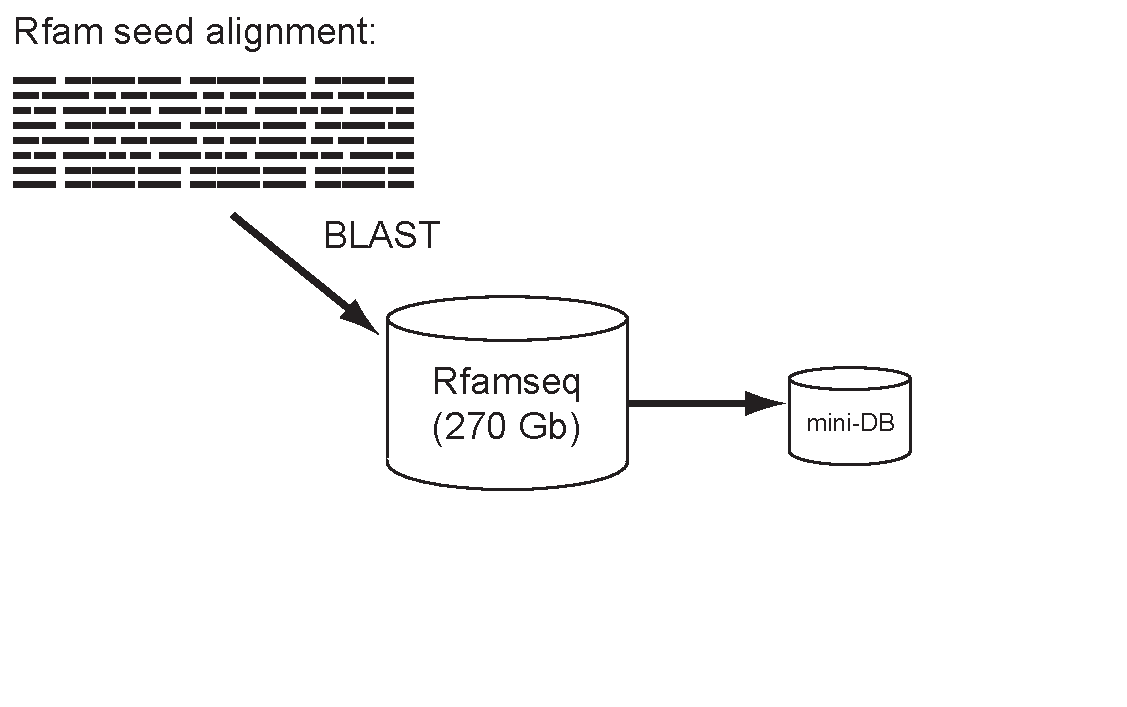
\includegraphics[width=8in]{figs/rfam-search-1}}

\vfill
\end{slide}
%%%%%%%%%%%%%%%%%%%%%%%%%%%%%%%%%%%%%%%%%%%%%%%%%%%%%%%%%%%%%%%%%%%%%%
\begin{slide}
\begin{center}

\textbf{Rfam used BLAST filters from 2003 to 2012}

\end{center}

\center{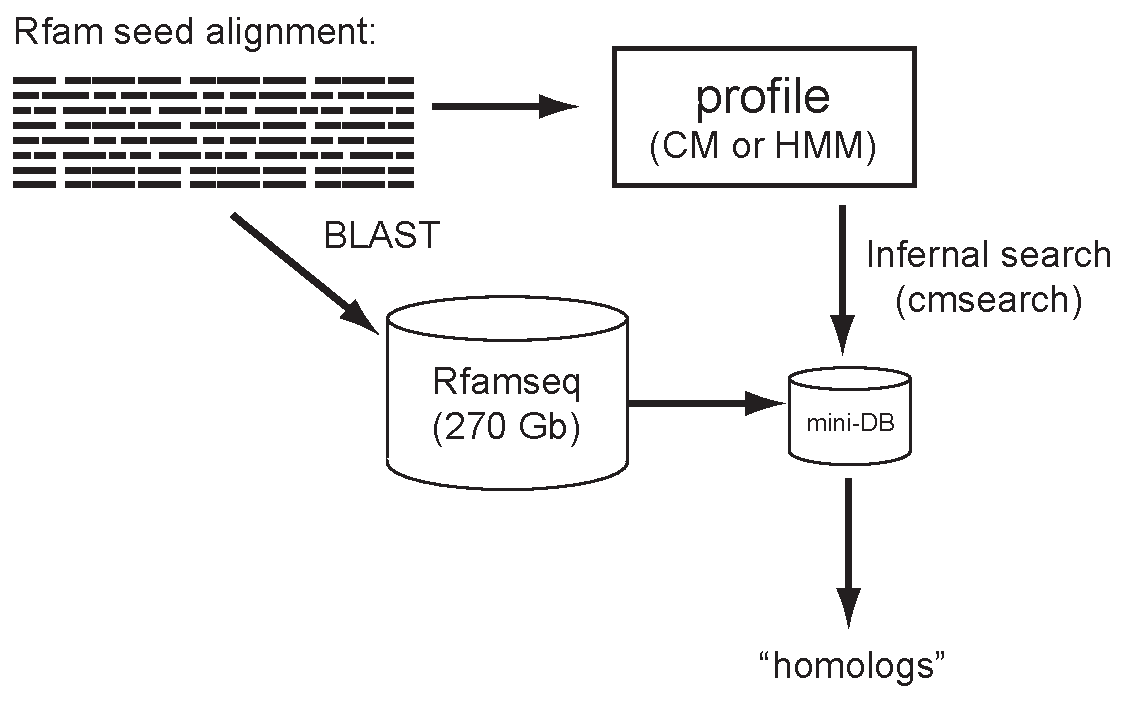
\includegraphics[width=8in]{figs/rfam-search-2}}

\vfill
\end{slide}
%%%%%%%%%%%%%%%%%%%%%%%%%%%%%%%%%%%%%%%%%%%%%%%%%%%%%%%%%%%%%%%%%%%%%%
\begin{slide}
\begin{center}

\textbf{Rfam 12.0 (2014)\footnote{Nawrocki, Burge et. al, NAR 2014, in press} first release without BLAST filtering}
\end{center}

\center{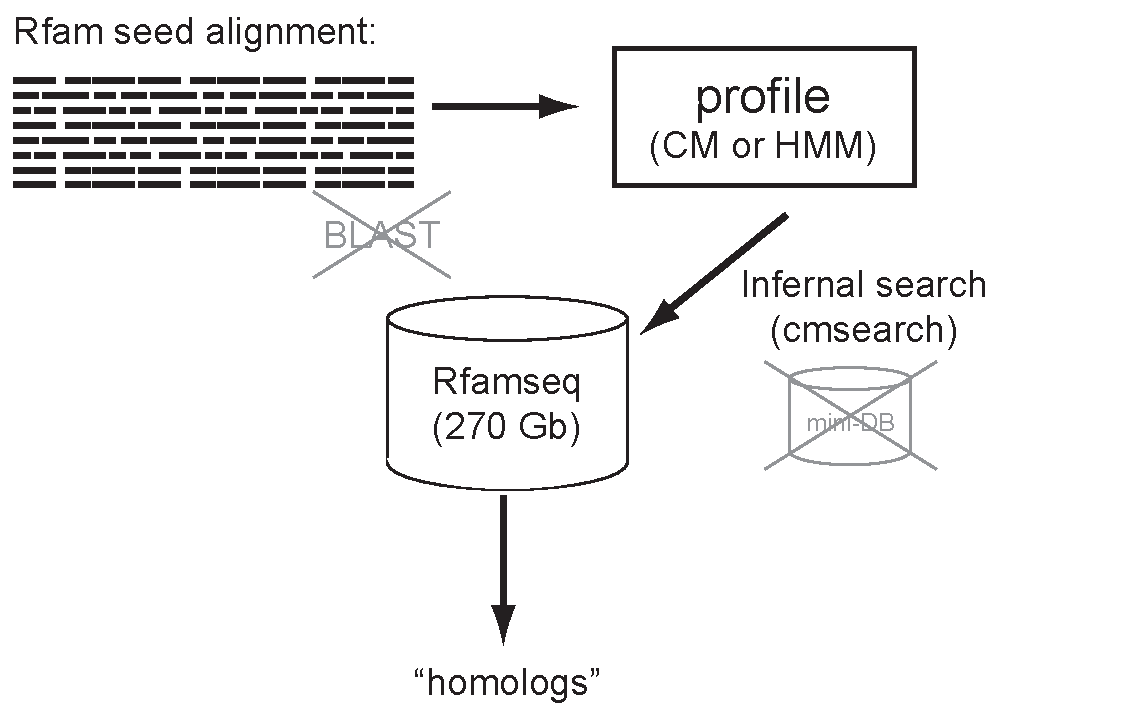
\includegraphics[width=8in]{figs/rfam-search-3}}

%\begin{center}
%\small
%Search results against Rfamseq for 200 random families:
%\begin{tabular}{l|rrr}
%strategy                   & time (h) & \# hits & \# unique hits \\ \hline
%Old (BLAST + Infernal 1.0) & 4069.8   &  179681 & 53 \\
%New (Infernal 1.1)         & 4222.2   &  201814 & 22312 \\
%\end{tabular}
%\end{center}

\vfill
\end{slide}
%%%%%%%%%%%%%%%%%%%%%%%%%%%%%%%%%%%%%%%%%%%%%%%%%%%%%%%%%%%%%%%%%%%%%%
\begin{slide}
\begin{center}

\textbf{Rfam 12.0 (2014)\footnote{Nawrocki, Burge et. al, NAR 2014, in press} first release without BLAST filtering}

\end{center}

\begin{center}
Search results against Rfamseq for 200 random families:

\medskip

\begin{tabular}{l|r|r|r}
strategy                   & time (h) & \# hits & \# unique hits \\ \hline
& & & \\
Old (BLAST + Infernal 1.0) & 4069.8   &  179,681 & 53 \\
& & & \\
New (Infernal 1.1)         & 4222.2   &  201,814 & 22,312 \\
\end{tabular}
\end{center}

\vfill
\end{slide}
%%%%%%%%%%%%%%%%%%%%%%%%%%%%%%%%%%%%%%%%%%%%%%%%%%%%%%%%%%%%%%%%%%%%%%
\begin{slide}

\large
\begin{center}
\large{\textbf{Acknowledgements}} \\

\vspace{0.5in}

\normalsize
%\begin{tabular}{llllll}
%Sean Eddy           & & & & & Michael Brent \\ 
%Elena Rivas         & & & & & Jeremy Buhler \\
%Tom Jones           & & & & & Justin Fay \\
%Diana Kolbe         & & & & & Jeff Gordon \\
%Seolkyoung Jung     & & & & & Rob Mitra \\
%Sergi Castellano    & & & & & Gary Stormo \\
%Fred Davis          & & & & & \\
%Lee Henry           & & & & & \\
%Michael Farrar      & & & & & \\
%Travis Wheeler      & & & & & \\
\begin{tabular}{l|l}
\textbf{Janelia} & \textbf{EBI (Rfam)} \\ \hline
{\bf Sean Eddy}     & {\bf Alex Bateman} \\
Elena Rivas         & {\bf Rob Finn} \\
Travis Wheeler      & {\bf Sarah Burge} \\ 
{\bf Tom Jones}     & {\bf Evan Floden} \\
Diana Kolbe         & John Tate \\
Seolkyoung Jung     & Jen Daub \\
Rob Finn            & \\
Jody Clements       & \\
Fred Davis          & \\
Lee Henry           & \\
Michael Farrar      & \\
\end{tabular}

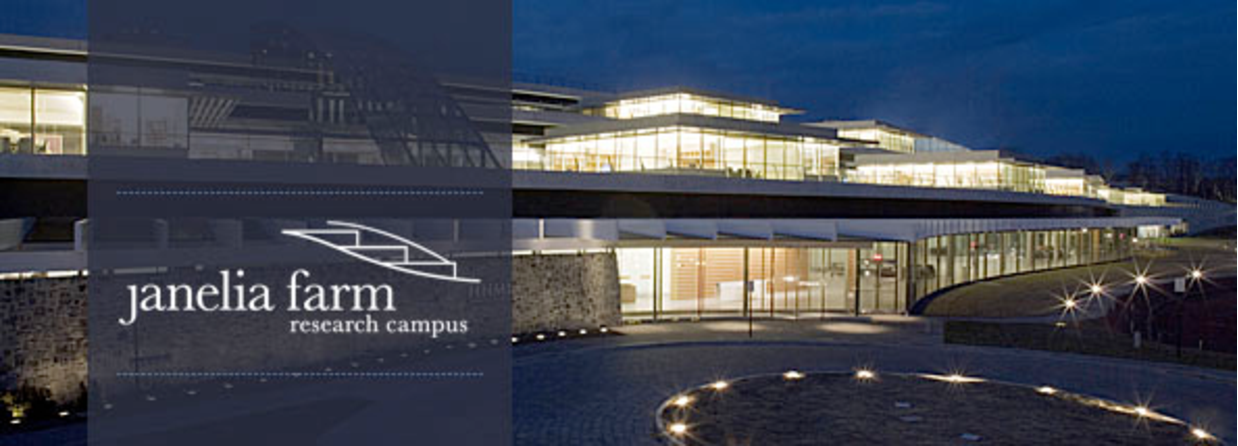
\includegraphics[height=3in]{figs/jfrc-banner1}

\end{center}

\vfill
\end{slide}
%%%%%%%%%%%%%%%%%%%%%%%%%%%%%%%%%%%%%%%%%%%%%%%%%%%%%%%%%%%%%%%%%%%%%%
\end{document}


\begin{tabular}{rl}
Rfam 1.0 to 11.0 (2003 to 2012): & Rfam used BLAST filters to accelerate Infernal \\
Rfam 12.0 (2014):                & first release without BLAST filters \\
\end{tabular}

Comparing sensitivity with and without BLAST filters for 200 randomly
chosen families:

%\begin{tabular}{rr|rr|rr}
% new (h): 4222.2
% old (h): 4069.8
% new # hits: 201814
% old # hits: 179681
% new uniq:    22312
% old uniq:       53
%\end{tabular}

\end{center}
